% !TEX program = xelatex
\documentclass[UTF8,fontset=fandol,a4paper,11pt]{ctexart}
\usepackage[margin=21mm,top=23mm,bottom=22mm,headheight=16pt]{geometry}
\usepackage{amsmath,amssymb,mathtools,bm}
\usepackage{tikz}
\usetikzlibrary{arrows.meta,calc,angles,quotes,patterns}
\usepackage{xcolor,booktabs,array,longtable,enumitem,fancyhdr,needspace}
\usepackage[unicode,hidelinks]{hyperref}
\definecolor{ink}{HTML}{24343C}
\definecolor{accent}{HTML}{166A70}
\definecolor{muted}{HTML}{65747A}
\definecolor{rulegray}{HTML}{D4DDE0}
\definecolor{warm}{HTML}{966037}
\color{ink}
\setlength{\parindent}{2em}
\setlength{\parskip}{4pt}
\linespread{1.12}
\AtBeginDocument{\setlength{\abovedisplayskip}{6pt plus 2pt minus 1pt}
\setlength{\belowdisplayskip}{6pt plus 2pt minus 1pt}
\setlength{\abovedisplayshortskip}{0pt plus 1pt}
\setlength{\belowdisplayshortskip}{4pt plus 1pt}}
\setlist[enumerate]{label=(\arabic*),leftmargin=2.3em,itemsep=3pt,topsep=4pt}
\setlist[itemize]{leftmargin=2em,itemsep=2pt,topsep=4pt}
\allowdisplaybreaks[1]
\setlength{\emergencystretch}{2em}
\setcounter{secnumdepth}{0}
\providecommand{\tightlist}{\setlength{\itemsep}{0pt}\setlength{\parskip}{0pt}}
\ctexset{section={format=\Large\bfseries\color{accent},beforeskip=10pt,afterskip=9pt},
subsection={format=\normalsize\bfseries\color{accent},beforeskip=10pt,afterskip=4pt},
subsubsection={format=\normalsize\bfseries,beforeskip=8pt,afterskip=3pt}}
\pagestyle{fancy}
\fancyhf{}
\fancyhead[L]{\small\color{muted}物理学难题集萃}
% 页眉仅保留书名；版本名称只在封面显示。
\fancyfoot[L]{\small\color{muted}\chapterlabel}
\fancyfoot[R]{\small\thepage}
\renewcommand{\headrulewidth}{0.4pt}
\renewcommand{\footrulewidth}{0pt}
\newcommand{\dd}{\mathop{}\!\mathrm{d}}
\newcommand{\vect}[1]{\bm{#1}}
\newcommand{\tagline}[1]{\noindent{\small\color{muted}#1}\par}
\newcommand{\result}[1]{\begin{equation*}\boxed{#1}\end{equation*}}
\newcommand{\figcaption}[1]{\par\vspace{2pt}{\small\color{muted}#1}\par}
\newcommand{\teach}[2]{\Needspace{4\baselineskip}\subsection*{讲解要点与追问}#1\par\smallskip\noindent\textbf{追问：}#2\par}
\newcommand{\workarea}{\par\vspace{7mm}\noindent{\small\color{muted}作答区}\par\vspace{4mm}
\noindent\textcolor{rulegray}{\rule{\linewidth}{0.3pt}}\par\vspace{16mm}
\noindent\textcolor{rulegray}{\rule{\linewidth}{0.3pt}}\par\vspace{16mm}
\noindent\textcolor{rulegray}{\rule{\linewidth}{0.3pt}}\par\vspace{16mm}
\noindent\textcolor{rulegray}{\rule{\linewidth}{0.3pt}}}
\tikzset{axis/.style={-{Stealth[length=2mm]},thin,color=muted},
motion/.style={-{Stealth[length=2.3mm]},thick,color=accent},
force/.style={-{Stealth[length=2.3mm]},thick,color=warm},
traj/.style={thick,color=accent},guide/.style={dashed,thin,color=muted},
object/.style={thick,color=ink},every node/.style={font=\small}}\widowpenalty=10000\clubpenalty=10000\displaywidowpenalty=10000\newcommand{\chapterlabel}{电磁学试题（一）}







\hypersetup{pdftitle={电磁学试题（一）·教师版},pdfauthor={}}

\begin{document}\pdfbookmark[0]{电磁学试题（一）}{cover}

\thispagestyle{empty}\vspace*{22mm}

\noindent{\Huge\bfseries 物理学难题集萃}\par\vspace{12mm}

\noindent{\LARGE 电磁学试题（一）}\par\vspace{12mm}

\noindent{\Large\color{accent}教师版}\par\vspace{9mm}

\noindent\textcolor{accent}{\rule{\linewidth}{1pt}}\par\vspace{9mm}

\noindent 第1--5题\par\vfill\clearpage

\pdfbookmark[1]{题目目录}{contents}\section*{题目目录}

\begin{longtable}{@{}r p{113mm} r@{}}\toprule 题号 & 题目 & 页码\\\midrule

\hyperref[q:1]{1} & \hyperref[q:1]{均匀电场中弹簧两端的带电小球} & \pageref{q:1} \\

\hyperref[q:2]{2} & \hyperref[q:2]{半无限导线向平面径向分流的磁场} & \pageref{q:2} \\

\hyperref[q:3]{3} & \hyperref[q:3]{水平磁场中下落带电球的临界轨迹} & \pageref{q:3} \\

\hyperref[q:4]{4} & \hyperref[q:4]{弱磁场中异号带电双体的质心摆线} & \pageref{q:4} \\

\hyperref[q:5]{5} & \hyperref[q:5]{带电容滑动双棒的充电与最终速度} & \pageref{q:5} \\

\bottomrule\end{longtable}

\clearpage

\pdfbookmark[2]{第 1 题 均匀电场中弹簧两端的带电小球}{q1}

\section*{第 1 题\quad 均匀电场中弹簧两端的带电小球}\label{q:1}


自由长度为$L$、劲度系数为$k$的轻弹簧，两端连接小球1、2，质量分别为$m_1,m_2$，正电荷分别为$Q_1,Q_2$。两球处于均匀电场中，场强$\boldsymbol E=E\hat x$沿初始连线由球1指向球2。初始两球静止、弹簧为自由长度。忽略重力、两球之间的电相互作用及辐射。
求此后两球间的最大距离，给出运动方程并讨论参数的不同情形。$L$足够大，保证压缩时两球始终不相碰、左右次序不交换。


\begin{center}\begin{minipage}{.98\linewidth}\centering
\begin{tikzpicture}[scale=.9,transform shape]

\draw[object] (.5,0)--(1,0)--(1.15,.2)--(1.45,-.2)--(1.75,.2)--(2.05,-.2)--(2.35,.2)--(2.65,-.2)--(2.95,.2)--(3.25,-.2)--(3.55,.2)--(3.85,-.2)--(4.15,.2)--(4.3,0)--(5,0);
\fill[accent!12] (.5,0) circle (.15);\draw[object] (.5,0) circle (.15);
\fill[warm!12] (5,0) circle (.15);\draw[object] (5,0) circle (.15);
\node[below,align=center] at (.5,-.3) {球1\\$m_1,Q_1$};
\node[below,align=center] at (5,-.3) {球2\\$m_2,Q_2$};
\draw[axis,<->] (.5,-1.9)--(5,-1.9) node[midway,below] {初始 $r=L$};
\draw[force] (1.3,1)--(4.2,1) node[midway,above] {$\boldsymbol E=E\hat x$};
\node at (2.7,.4) {$k$};

\end{tikzpicture}
\figcaption{图电试1.1\quad 初始弹簧为自由长度，电场由球1指向球2。}
\end{minipage}\end{center}

\Needspace{8\baselineskip}

\pdfbookmark[3]{题型定位}{q1-h0}

\subsection*{题型定位}

均匀场中两体系统的质心与相对运动分离。外电场驱动整体加速，电荷质量比的不一致才驱动弹簧伸缩。先用相对驱动力的符号判断伸长或压缩，再选取真正的最大间距。

图C逐一写出两球在质心系中的恢复力，由此求出与相对方程相同的频率和确定的相位关系。图D再用相对有效势的两个转点判断哪一端是最大间距。这里的平衡位置属于加速质心系，地面观察到的每球位置还要加同一个$X(t)$。

\Needspace{8\baselineskip}

\pdfbookmark[3]{知识点}{q1-h1}

\subsection*{知识点}

\begin{itemize}
\item 总外力决定质心加速度，质心参考系在本题中加速。
\item 相对坐标与约化质量$\mu=m_1m_2/(m_1+m_2)$。
\item 恒驱动力平移简谐平衡点，初始零速度确定相位。
\item 伸长、等长、压缩三种情形与接触约束。
\end{itemize}

由$\xi_1=-m_2r/M,\xi_2=m_1r/M$可知，两球的内部振动由同一个相对坐标决定；质量加权位移及速度和都为零。相对电功为$F_d\Delta r$，整体电功为$(Q_1+Q_2)E\Delta X$，两者分别进入约化运动和质心运动。严格不接触的条件是全程$r>0$；求得的长度范围应满足这个条件。

\Needspace{8\baselineskip}

\pdfbookmark[3]{物理图像}{q1-h2}

\subsection*{物理图像}

图电试1.1固定球的左右次序和电场方向。解图电试1.1A只分析间距$r$及平衡位置$L+\delta$，把整体加速与伸缩分开。解图电试1.1B画两个有符号的$\delta$示例，显示压缩时$L$已经是最大间距。地面轨迹由各球的质心系坐标叠加$a_Ct^2/2$得到，振动中心随质心运动。

图C上下两组的质量比相同，分别取$\delta>0$和$\delta<0$。每一行的$C$都是同一加速参考系中的原点，平衡行对应$\omega t=\pi/2$，另一转点行对应$\pi$。图D示例取$\delta>0$，能量线两端在$r=L$与$L+2\delta$；图B的压缩分支取$\delta<0$，后一转点的长度更小。

\Needspace{8\baselineskip}

\pdfbookmark[3]{解题入口}{q1-h3}

\subsection*{解题入口}

分别写两球方程，先相加得到质心，再用加速度相减得到相对方程。让学生用$Q_2/m_2-Q_1/m_1$先判断初始伸缩方向，写出$r_e$以后再用初始条件求余弦相位。最后从$1-\cos\omega t$的范围读出最大间距。

若学生选择质心法，要求先写$-m_i a_C$，再用$m_1\xi_1+m_2\xi_2=0$消去另一位置，最后才求平衡点。在图C中，右球位于质心右侧，其平衡坐标取正号。若选择相对法，则先求有向$\delta$，到求振幅时才取绝对值；从范围式中同时读出$r_{\min}$，检查题设是否允许完整运动。

\Needspace{8\baselineskip}

\pdfbookmark[3]{标准解法}{q1-h4}

\subsection*{标准解法}


图电试1.1取球1在左、球2在右，定义
\[
M=m_1+m_2,\quad \mu=\frac{m_1m_2}{M},\quad
r=x_2-x_1>0,\quad X=\frac{m_1x_1+m_2x_2}{M}.
\]
两条牛顿方程为
\[
m_1\ddot x_1=Q_1E+k(r-L),\qquad
m_2\ddot x_2=Q_2E-k(r-L).
\]
两式相加给质心运动：
\[
\boxed{\ddot X=\frac{(Q_1+Q_2)E}{M}=a_C}.
\]
两加速度相减并乘约化质量，得
\[
\mu\ddot r=
\frac{m_1Q_2-m_2Q_1}{M}E-k(r-L).
\]
记相对驱动力、平衡伸长和振动角频率为
\[
F_d=\frac{m_1Q_2-m_2Q_1}{M}E,\quad
\delta=\frac{F_d}{k},\quad
\omega=\sqrt{\frac{k}{\mu}}.
\]
\begin{center}\begin{minipage}{.98\linewidth}\centering
\begin{tikzpicture}[scale=.85,transform shape]

\draw[axis] (0,0)--(6,0) node[right] {$r$};
\draw[axis] (0,-1.3)--(0,2.8) node[above] {$F_{\rm rel}$};
\draw[traj] (1,2)--(5,-1);
\draw[guide] (3.667,0)--(3.667,-.8);
\node[below] at (3.667,-.8) {$r_e=L+\delta$};
\draw[guide] (2.5,0)--(2.5,.875);
\node[below] at (2.5,0) {$L$};
\node[above right] at (2.5,.875) {$F_d$};
\node at (4.1,2.5) {$F_{\rm rel}=-k(r-r_e)$};
\node at (3,-1.8) {示例 $\delta>0$；质心另有加速度 $a_C$};

\end{tikzpicture}
\figcaption{解图电试1.1A\quad 相对驱动力移动平衡点，斜率仍为负k。}
\end{minipage}\end{center}
解图电试1.1A把相对坐标的平衡点标为$r_e=L+\delta$。方程写成
\[
\ddot{(r-r_e)}+\omega^2(r-r_e)=0.
\]
由$r(0)=L,\dot r(0)=0$，
\[
\boxed{r(t)=L+\delta(1-\cos\omega t)}.
\]
若初始质心位置选为零、质心初速为零，地面系两球位置为
\[
\boxed{x_1(t)=\frac12a_Ct^2-\frac{m_2}{M}r(t),\qquad
x_2(t)=\frac12a_Ct^2+\frac{m_1}{M}r(t)}.
\]
初始$x_1=-m_2L/M,x_2=m_1L/M$，质量加权平均及相对初速都满足题设。球在质心系中的振幅分别为$m_2|\delta|/M,m_1|\delta|/M$，质心在地面系中作加速度为$a_C$的匀加速运动。

\begin{center}\begin{minipage}{.98\linewidth}\centering
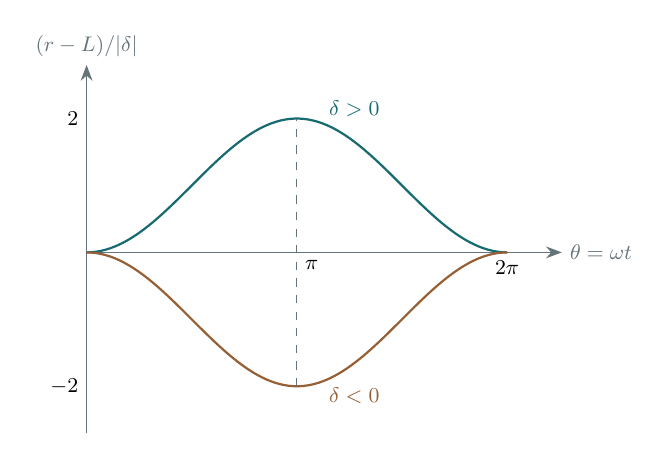
\begin{tikzpicture}[scale=.85,transform shape]

\draw[axis] (0,0)--(7.1,0) node[right] {$\theta=\omega t$};
\draw[axis] (0,-2.7)--(0,2.8) node[above] {$(r-L)/|\delta|$};
\draw[traj,domain=0:6.2832,samples=90] plot (\x,{1-cos(deg(\x))});
\draw[thick,color=warm,domain=0:6.2832,samples=90] plot (\x,{-1+cos(deg(\x))});
\draw[guide] (3.14159,-2)--(3.14159,2);
\node[left] at (0,2) {$2$};\node[left] at (0,-2) {$-2$};
\node[below right] at (3.14159,0) {$\pi$};
\node[below] at (6.2832,0) {$2\pi$};
\node[above,color=accent] at (4,1.9) {$\delta>0$};
\node[below,color=warm] at (4,-1.9) {$\delta<0$};

\end{tikzpicture}
\figcaption{解图电试1.1B\quad 伸长分支超过L，压缩分支的最大值已是初始L。}
\end{minipage}\end{center}
解图电试1.1B分别画$\delta>0$和$\delta<0$的间距变化，二者都从$L$以零斜率出发。
\begin{enumerate}
\item 若$m_1Q_2>m_2Q_1$，球2的自由电加速度较大，弹簧开始伸长。间距在$L$与$L+2\delta$之间变化，故
\[
\boxed{r_{\max}=L+
\frac{2(m_1Q_2-m_2Q_1)E}{k(m_1+m_2)}}.
\]
最大值首次出现在$t=\pi/\omega$。
\item 若$m_1Q_2=m_2Q_1$，两球自由电加速度相等，相对驱动力为零，弹簧始终不伸缩，$r(t)=L$。
\item 若$m_1Q_2<m_2Q_1$，球1的自由电加速度较大，弹簧开始压缩。间距范围为$L+2\delta\le r\le L$，因此初始长度$L$就是间距的最大值。题设的“不相碰”要求$L+2\delta>0$。
\end{enumerate}
合写为
\[
\boxed{r_{\max}=L+\frac{2E}{kM}
\max(m_1Q_2-m_2Q_1,0)}.
\]
\textbf{把相对运动还原为两球的振动。}图C在同一质心坐标中列出初始、平衡和另一转点的位置。令$\xi_i=x_i-X$，则$m_1\xi_1+m_2\xi_2=0$，两球分别位于$-m_2r/M$和$m_1r/M$。在随质心加速而不转动的参考系中，每球增加惯性力$-m_i a_C$，合力为
\[
F_1^{(C)}=Q_1E+k(r-L)-m_1a_C=-F_d+k(r-L),
\qquad F_2^{(C)}=F_d-k(r-L).
\]
由质心约束消去另一球的位置，得到
\[
F_1^{(C)}=-\frac{kM}{m_2}(\xi_1-\xi_{1e}),\quad
F_2^{(C)}=-\frac{kM}{m_1}(\xi_2-\xi_{2e}),
\]
\[
\xi_{1e}=-\frac{m_2}{M}(L+\delta),\qquad
\xi_{2e}=\frac{m_1}{M}(L+\delta).
\]
平衡时两球相对于加速质心保持固定位置，在地面系中仍共同具有$a_C$的加速度，各球所受合力为$m_i a_C$。两式分别除以各自质量，角频率均为$\sqrt{kM/(m_1m_2)}$，与相对坐标方法一致。

初始质心位置取零时，$\xi_1(0)=-m_2L/M$、$\xi_2(0)=m_1L/M$，故各自离平衡点的有向位移为
\[
\xi_1(0)-\xi_{1e}=\frac{m_2}{M}\delta,\qquad
\xi_2(0)-\xi_{2e}=-\frac{m_1}{M}\delta.
\]
两球初始相对速度为零，因而
\[
\xi_1(t)=\xi_{1e}+\frac{m_2\delta}{M}\cos\omega t,\qquad
\xi_2(t)=\xi_{2e}-\frac{m_1\delta}{M}\cos\omega t.
\]
两球同频、反相，质量加权位移和始终为零，初始相位由同一组初值确定。各球振幅为$A_1=m_2|\delta|/M$、$A_2=m_1|\delta|/M$。到$t=\pi/\omega$时，每球走到相反转点，离开初始位置的距离为$2A_i$。若$\delta>0$，两球向外分开，间距增加$2(A_1+A_2)=2\delta$；若$\delta<0$，这组位移使两球靠近，对应最小间距。图C中压缩分支的两个平衡点均在初始位置内侧，伸长分支则均在外侧。

\begin{center}\begin{minipage}{.98\linewidth}\centering
\begin{tikzpicture}[scale=.87,transform shape]
\draw[guide] (0,.6)--(0,-6.1);\node[above]at(0,.6){$C:\ \xi=0$};
\node[anchor=east]at(-2.3,.05){$\delta>0$};\node[anchor=east]at(-2.3,-3.55){$\delta<0$};
\foreach \y/\a/\b/\lab in {0/-1/2/{初始},-1/-1.2/2.4/{平衡},-2/-1.4/2.8/{另一转点},-3.6/-1/2/{初始},-4.6/-.8/1.6/{平衡},-5.6/-.6/1.2/{另一转点}}{
 \draw[axis](-1.8,\y)--(3.35,\y);\node[anchor=east]at(-1.9,\y){\lab};
 \fill[accent](\a,\y)circle(2pt)node[above]{$1$};\fill[warm](\b,\y)circle(2pt)node[above]{$2$};
}
\node[right]at(3.5,0){$r=L$};\node[right]at(3.5,-1){$r=L+\delta$};\node[right]at(3.5,-2){$r=L+2\delta$};
\node[right]at(3.5,-3.6){$r=L$};\node[right]at(3.5,-4.6){$r=L+\delta$};\node[right]at(3.5,-5.6){$r=L+2\delta$};
\node[below]at(.5,-6.15){示例 $m_1:m_2=2:1,\ L=3,\ |\delta|=0.6$，各长度共用同一单位};
\end{tikzpicture}
\figcaption{解图电试1.1C\quad 质量加权的质心位置、平衡位置与同步转点}
\end{minipage}\end{center}

\textbf{能量中的整体项与伸缩项。}图D按相对坐标画出有效势能。由坐标变换直接展开两球动能，可得
\[
T=\frac12M\dot X^2+\frac12\mu\dot r^2,
\qquad Q_1x_1+Q_2x_2=(Q_1+Q_2)X+\frac{m_1Q_2-m_2Q_1}{M}r.
\]
上述坐标恒等式在$E=0$时仍成立，电场所做的功为零。均匀电场对整体坐标的功为$(Q_1+Q_2)E\,\Delta X$，对相对坐标的功为$F_d\Delta r$。相对运动因而满足
\[
\frac12\mu\dot r^2+\frac12k(r-L)^2-F_d(r-L)=0,
\]
初始常数已按$r=L,\dot r=0$取定。配方后，相对运动的有效能量为
\[
\frac12\mu\dot r^2+\frac12k(r-L-\delta)^2
=\frac12k\delta^2.
\]
图D的水平能量线与抛物线交于$r=L$和$r=L+2\delta$。弹簧达到最大形变量时相对动能为零，系统仍保留同一时刻的质心动能。计算两球全部动能时，还须计入电场对质心所做的功。

\begin{center}\begin{minipage}{.98\linewidth}\centering
\begin{tikzpicture}[scale=.86,transform shape]
\draw[axis](-.2,0)--(5.9,0)node[right]{$u=(r-L)/\delta$};
\draw[axis](0,-.2)--(0,3.3)node[above right]{$V_{\rm eff}/(k\delta^2/2)$};
\draw[traj,domain=0:2.15,samples=70]plot({2.5*\x},{2*(\x-1)^2});
\draw[guide](0,2)--(5.45,2)node[right]{$\mathcal H_{\rm rel}=k\delta^2/2$};
\fill[accent](0,2)circle(2pt);\fill[accent](5,2)circle(2pt);
\node[above right]at(0,2){初始 $r=L$};\node[above left]at(5,2){另一转点 $r=L+2\delta$};
\node[below]at(2.5,0){$1$};\node[below]at(5,0){$2$};\node[left]at(0,2){$1$};
\node[below]at(2.5,-.6){图示 $\delta>0$；最低点为 $r_e=L+\delta$};
\end{tikzpicture}
\figcaption{解图电试1.1D\quad 相对有效势能的两个转点，图示 $\delta>0$ 的分支}
\end{minipage}\end{center}

两转点之间的间距范围可统一写成
\[
r_{\min}=L+2\min(\delta,0),\qquad
r_{\max}=L+2\max(\delta,0).
\]
题设要求$r_{\min}>0$。压缩分支只有在$L+2\delta>0$时才允许沿本模型走完整周期；等号已经发生接触。$\delta=0$时所有时刻都保持$r=L$，按恒定间距处理。两球共同加速与内部长度不变可以同时成立。



\Needspace{8\baselineskip}

\pdfbookmark[3]{关键洞察}{q1-h5}

\subsection*{关键洞察}

相对驱动由电荷质量比的差决定，总电荷决定质心加速，分别进入$r(t)$与$X(t)$的方程。对$\delta<0$，两球离平衡位置虽都有非零振幅，初始状态却已处于最大间距；把两振幅一律加到$L$上会选错转向点。

两振幅之和为$|\delta|$，相对驱动力的符号决定两球从初始长度开始伸长还是压缩。图D的两个转点处相对动能为零，质心速度仍由整体运动方程给出。给两球同时加同一个外部加速度，只改变$X(t)$而不改变$r(t)$，可用这一性质区分整体力和差动力。

\Needspace{8\baselineskip}

\pdfbookmark[3]{易错点}{q1-h6}

\subsection*{易错点}

\begin{itemize}
\item 在加速质心系漏惯性力，直接让每球只受电力和弹簧力。
\item 只用总电荷计算弹簧伸长，没有比较电荷质量比。
\item 把初始长度$L$误作场中平衡长度。
\item 求振幅时取绝对值后丢掉压缩分支，错误给所有情形同一增距公式。
\item 压缩幅度超过$L$仍让两球穿过彼此，超出题设模型。
\end{itemize}

图C右球的平衡坐标为$+m_1(L+\delta)/M$；初位减去平衡位置，得到有向初始位移$-m_1\delta/M$。两球在同一时刻到达相反转点，相对速度同时为零；求间距时使用这对同时发生的位置。题目中的$L$是弹簧自由长度；准备到场中相对平衡长度后再释放，初态已经改变。

\Needspace{8\baselineskip}

\pdfbookmark[3]{课堂讲解建议}{q1-h7}

\subsection*{课堂讲解建议}

先提出两个极端：两球电荷质量比相等，以及球2几乎不带电。前者应完全不伸缩，后者在电场向右时先压缩。用这两个预测检查相对方程的符号。得到$r(t)$后，请学生在$t=0$和$\pi/\omega$分别标出球的位置，解释哪一个时刻才是最大间距。最后追问质心是否静止，要求把整体加速与内部振动分别说清。

请学生在图C的每一行核算$m_1\xi_1+m_2\xi_2$，再标两球在前半周期的运动箭头。用图D追问“此时哪些动能为零”，要求分别回答质心与相对项。最后比较场中平衡准备、运动中反转电场和半周期电场脉冲三个初值问题，让学生把切换瞬间的$r,\dot r$作为下一阶段初值。

\Needspace{8\baselineskip}

\pdfbookmark[3]{变式训练}{q1-h8}

\subsection*{变式训练}

\begin{enumerate}
\Needspace{34\baselineskip}
\item 取$m_1=m_2=m,Q_1=Q,Q_2=3Q$，其余初态与主解相同，求$r(t)$、第一次最大间距及两球相对质心的振幅。
\textbf{解：}对一般等质量情形，$\mu=m/2,\omega=\sqrt{2k/m},\delta=(Q_2-Q_1)E/(2k)$；$Q_2>Q_1$对应伸长，相等电荷则共同以$QE/m$加速。本问取$Q_1=Q,Q_2=3Q$。图V1中两球质量相同，而初始电力分别为$QE$和$3QE$。约化质量$m/2$，相对驱动力为$QE$，所以
\[\delta=\frac{QE}{k},\quad\omega=\sqrt{\frac{2k}{m}},\quad r=L+\frac{QE}{k}(1-\cos\omega t).\]
球2的自由加速度较大，选择伸长分支，$r_{\max}=L+2QE/k$，第一次发生在$t=\pi\sqrt{m/(2k)}$。两球在质心系的振幅各为$QE/(2k)$，质心加速度却为$2QE/m$。图V1中两电力的长度比为1比3；两振幅则由相同的质量和质心约束确定，大小相等。
\begin{center}\begin{minipage}{.98\linewidth}\centering
\begin{tikzpicture}[scale=.85,transform shape]
\draw[object](.5,0)--(5,0);\fill[accent](.5,0)circle(3pt)node[below]{$m,Q$};\fill[warm](5,0)circle(3pt)node[below]{$m,3Q$};
\node[above]at(2.7,0){$k,L$};\draw[force](.5,.5)--(1.5,.5)node[midway,above]{$QE$};\draw[force](5,.5)--(8,.5)node[midway,above]{$3QE$};\node[below]at(4,-.8){初始弹簧力为零；两球振幅均为 $\delta/2$};
\end{tikzpicture}
\figcaption{变图电试1.1V1}
\end{minipage}\end{center}

\Needspace{34\baselineskip}
\item 相对初速改为$w_0=\omega\delta$，其中$\delta>0$，初长仍为$L$。求极值和第一次最大间距时刻，并给出不碰撞条件。
\textbf{解：}一般相对初速为$w_0$时，$r=L+\delta-\delta\cos\omega t+(w_0/\omega)\sin\omega t$，其振幅为$\sqrt{\delta^2+(w_0/\omega)^2}$，最大长度为$L+\delta+\sqrt{\delta^2+(w_0/\omega)^2}$，最小长度由平衡长度减去同一振幅给出。本问取$w_0=\omega\delta$，于是图V2取$u=(r-r_e)/\delta,v=\dot r/(\omega\delta)$，初点为$(-1,1)$。初值解为
\[r-r_e=\delta(-\cos\omega t+\sin\omega t)=\sqrt2\delta\sin(\omega t-\pi/4).\]
故$r_{\max}=L+(1+\sqrt2)\delta$，$r_{\min}=L+(1-\sqrt2)\delta$，要求$L>(\sqrt2-1)\delta$。第一次最大值在$\omega t=3\pi/4$；零相对初速的情形在$\pi$达到最大值，相对初速改变了初相位。图V2的相轨迹为$u^2+v^2=2$，沿顺时针转动；右端点给长度最大，初点不在横轴上。
\begin{center}\begin{minipage}{.98\linewidth}\centering
\begin{tikzpicture}[scale=.85,transform shape]
\draw[axis](-1.9,0)--(2,0)node[right]{$u$};\draw[axis](0,-1.8)--(0,2)node[above]{$v$};\draw[traj](0,0)circle(1.414214);\fill[warm](-1,1)circle(2pt)node[above left]{初点 $(-1,1)$};\fill[accent](1.414214,0)circle(2pt)node[below right]{$\sqrt2$};\draw[motion](1.35,.42)arc[start angle=17.3,end angle=-15,radius=1.414];
\end{tikzpicture}
\figcaption{变图电试1.1V2}
\end{minipage}\end{center}

\Needspace{34\baselineskip}
\item 从主解的$\delta>0$初态出发，在$t_s=\pi/\omega$瞬时将电场反向。求切换后的间距范围，判断能否把“初态重做实验”的分支交换直接用于这一过程。
\textbf{解：}从自由长度和零相对初速重新开始的反向实验中，$F_d,\delta$变号，伸长与压缩分支交换，质心加速度反向而$\omega=\sqrt{k/\mu}$保持不变。本问则在运动到转点后反向，继承这一时刻的初值。图V3在切换处继承$r=L+2\delta,\dot r=0$；新驱动为$-F_d$、新平衡长度为$L-\delta$，故令$s=t-t_s\ge0$，
\[r(s)=L-\delta+3\delta\cos\omega s.\]
切换后的范围为$L-4\delta\le r\le L+2\delta$，要求$L>4\delta$。从自由长度重新开始的反向实验振幅只有$\delta$，本过程却相对新平衡点偏离$3\delta$；区别来自初值。图V3横轴为$\omega t/\pi$，切换点是1，随后在2处达到最小值。
\begin{center}\begin{minipage}{.98\linewidth}\centering
\begin{tikzpicture}[scale=.85,transform shape]
\draw[axis](0,-2.2)--(0,1.6)node[above]{$(r-L)/\delta$};\draw[axis](0,0)--(3.4,0)node[right]{$\omega t/\pi$};\draw[traj,domain=0:pi,samples=45]plot({\x/pi},{.5*(1-cos(deg(\x)))});\draw[thick,color=warm,domain=pi:3*pi,samples=90]plot({\x/pi},{.5*(-1+3*cos(deg(\x-pi)))});\draw[guide](1,-2.1)--(1,1.3);\node[above]at(1,1.3){反向};\node[left]at(0,1){$2$};\node[left]at(0,-2){$-4$};\node[below]at(2,0){$2$};
\end{tikzpicture}
\figcaption{变图电试1.1V3}
\end{minipage}\end{center}

\Needspace{34\baselineskip}
\item 先把相对状态准备为$r=L+\delta,\dot r=0$，$\delta>0$，质心初速为零。比较释放时保持电场和同时撤去电场两种安排，求其后的相对振动。
\textbf{解：}图V4中的初始长度是场中平衡长度。保持电场时，$F_d-k\delta=0$，相对长度不变，质心以$a_C$加速。若撤去电场，平衡长度立即变回$L$，但$r,\dot r$连续，因而
\[r=L+\delta\cos\omega t,\qquad L-\delta\le r\le L+\delta.\]
此时要求$L>\delta$，质心保持静止，内部机械能为$k\delta^2/2$。图V4以$(r-L)/\delta$画两种结果，水平线对应保留电场，余弦线对应撤场；“从平衡释放”要同时指明哪个外场仍然存在。
\begin{center}\begin{minipage}{.98\linewidth}\centering
\begin{tikzpicture}[scale=.85,transform shape]
\draw[axis](0,-1.3)--(0,1.6)node[above right]{$(r-L)/\delta$};\draw[axis](0,0)--(6.7,0)node[right]{$\omega t$};\draw[traj](0,1)--(6.28,1)node[right]{保留电场};\draw[thick,color=warm,domain=0:2*pi,samples=70]plot(\x,{cos(deg(\x))});\node[below,color=warm]at(3.2,-1){撤去电场};\node[below]at(6.28,0){$2\pi$};
\end{tikzpicture}
\figcaption{变图电试1.1V4}
\end{minipage}\end{center}

\Needspace{34\baselineskip}
\item 已知$m_1,m_2,k,E,L$，测得初态如主解时$r_{\max}=L+\Delta L$，其中$\Delta L>0$。求两球电荷质量比的差。若只测得$r_{\max}=L$，能否判断两电荷质量比相等？
\textbf{解：}图V5以有向$\delta$为横轴、最大增距为纵轴。正增距选择伸长分支，$\delta=\Delta L/2$，所以
\[m_1Q_2-m_2Q_1=\frac{kM\Delta L}{2E},\qquad
\frac{Q_2}{m_2}-\frac{Q_1}{m_1}=\frac{kM\Delta L}{2E m_1m_2}.\]
若最大值等于$L$，只能推出$\delta\le0$，无法区分等长与压缩。还要测最小长度：若$r_{\min}<L$，便有$\delta=(r_{\min}-L)/2<0$；若两极值均为$L$，才有差为零。反求电荷时，最大值曲线的水平部分不提供唯一的压缩幅度。
\begin{center}\begin{minipage}{.98\linewidth}\centering
\begin{tikzpicture}[scale=.85,transform shape]
\draw[axis](-2,0)--(3,0)node[right]{$\delta$};\draw[axis](0,-.2)--(0,2.9)node[above right]{$r_{\max}-L$};\draw[traj](-1.7,0)--(0,0)--(1.3,2.6);\node[above]at(-1,.15){压缩分支};\node[right]at(1,1.7){斜率 $2$};\node[below]at(0,0){$0$};
\end{tikzpicture}
\figcaption{变图电试1.1V5}
\end{minipage}\end{center}

\Needspace{34\baselineskip}
\item 设$m_2Q_1>m_1Q_2$，两球可视作质点。求完整周期内严格不相碰所允许的电场上限，并说明等号的意义。
\textbf{解：}记$D=m_2Q_1-m_1Q_2>0$，有$\delta=-DE/(kM)$，图V6画$r_{\min}/L$。严格不接触要求
\[L-\frac{2DE}{kM}>0,\qquad 0\le E<E_c=\frac{kML}{2D}.\]
在$E=E_c$时，$\omega t=\pi$处$r=0,\dot r=0$，两球恰好接触；严格不接触对应上式的开区间。若两球有不可忽略半径，接触中心距为$b>0$，应改为$L-2DE/(kM)>b$，即$E<kM(L-b)/(2D)$，且$L>b$。图V6横轴处的空圈表示达到接触，严格不碰撞的取值位于空圈左侧。
\begin{center}\begin{minipage}{.98\linewidth}\centering
\begin{tikzpicture}[scale=.85,transform shape]
\fill[warm!10](3,0)rectangle(3.9,2.4);\draw[axis](0,0)--(4.1,0)node[right]{$E/E_c$};\draw[axis](0,-.1)--(0,2.7)node[above right]{$r_{\min}/L$};\draw[traj](0,2)--(3,0);\draw[object,fill=white](3,0)circle(2.5pt);\node[left]at(0,2){$1$};\node[below]at(3,0){$1$};\node[rotate=90]at(3.55,1.2){接触或模型失效};\node at(1.2,.35){严格不碰撞};
\end{tikzpicture}
\figcaption{变图电试1.1V6}
\end{minipage}\end{center}

\Needspace{34\baselineskip}
\item 在主解的电力之外，每球另受沿$x$的力$m_i g_x$，其中有向常量$g_x$对两球相同。初始仍为自由长度、两球静止。求$r(t)$与质心运动，并讨论$g_x=-a_C$。
\textbf{解：}图V7把附加力按质量成比例画出。两球加速度相减时，两个$g_x$相消，所以相对驱动仍为
\[\mu\left[\left(\frac{Q_2E}{m_2}+g_x\right)-\left(\frac{Q_1E}{m_1}+g_x\right)\right]=F_d.\]
因此$r=L+\delta(1-\cos\omega t)$和最大、最小间距都不变，质心则满足$X=(a_C+g_x)t^2/2$。若$g_x=-a_C$，质心可静止而内部仍振动，只要电荷质量比不同；相反，电荷质量比相等时两球即使整体加速也不伸缩。共同加速度与相对差动力是两个独立条件。
\begin{center}\begin{minipage}{.98\linewidth}\centering
\begin{tikzpicture}[scale=.85,transform shape]
\fill[accent](0,0)circle(3pt)node[left]{$m_1,Q_1$};\fill[warm](4,0)circle(3pt)node[left]{$m_2,Q_2$};\draw[force](0,.3)--(1.7,.3)node[midway,above]{$Q_1E$};\draw[force](4,.3)--(6,.3)node[midway,above]{$Q_2E$};\draw[motion](0,-.3)--(1.7,-.3)node[midway,below]{$m_1g_x$};\draw[motion](4,-.3)--(6,-.3)node[midway,below]{$m_2g_x$};\node[below]at(2.5,-1.1){图示 $g_x>0$；附加加速度相同，力一般不同};
\end{tikzpicture}
\figcaption{变图电试1.1V7}
\end{minipage}\end{center}

\Needspace{34\baselineskip}
\item 从主解初态起施加恒定电场，持续时间$T$后撤场，理想切换时$r,\dot r$连续。求撤场后自由伸缩的振幅，并讨论$T=\pi/\omega$和$2\pi/\omega$。
\textbf{解：}切换前$r-L=\delta(1-\cos\omega T)$、$\dot r=\delta\omega\sin\omega T$。撤场后的平衡长度是$L$，所以
\[A_T=\sqrt{[r(T)-L]^2+[\dot r(T)/\omega]^2}=2|\delta\sin(\omega T/2)|.\]
图V8给$A_T/|\delta|$随脉冲时长的变化，撤场后的长度范围为$L\pm A_T$，需$L>A_T$。半周期脉冲给振幅$2|\delta|$；整周期脉冲给零振幅，内部回到自由长度且相对速度为零，但质心仍获得速度$a_CT$。半周期时弹簧储能为$2k\delta^2$，整周期时内部能量恢复为零；质心动能由同一时刻的质心速度另行计算。
\begin{center}\begin{minipage}{.98\linewidth}\centering
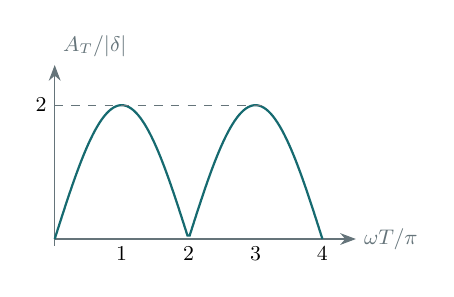
\begin{tikzpicture}[scale=.85,transform shape]
\draw[axis](0,0)--(4.5,0)node[right]{$\omega T/\pi$};\draw[axis](0,-.1)--(0,2.6)node[above right]{$A_T/|\delta|$};\draw[traj,domain=0:4*pi,samples=120]plot({\x/pi},{2*abs(sin(deg(\x/2)))});\foreach \x in{1,2,3,4}{\node[below]at(\x,0){$\x$};}\node[left]at(0,2){$2$};\draw[guide](0,2)--(3.2,2);
\end{tikzpicture}
\figcaption{变图电试1.1V8}
\end{minipage}\end{center}
\end{enumerate}

\Needspace{13\baselineskip}

\pdfbookmark[2]{第 2 题 半无限导线向平面径向分流的磁场}{q2}

\section*{第 2 题\quad 半无限导线向平面径向分流的磁场}\label{q:2}


稳恒电流$I$沿负$x$半轴流向原点$O$，到达$x=0$的无限大平面后均匀向各径向散开。平面上的面电流密度为
\[
\boldsymbol K(\rho)=\frac{I}{2\pi\rho}\hat{\boldsymbol\rho},\qquad \rho>0.
\]
求右半空间$x>0$、左半空间$x<0$以及平面两侧的磁场。规定$\hat{\boldsymbol\phi}$绕$+x$轴按右手方向，真空磁导率为$\mu_0$。另说明理想电流面上以及理想细导线轴线上的场应怎样理解。


\begin{center}\begin{minipage}{.98\linewidth}\centering
\begin{tikzpicture}[scale=.9,transform shape]

\fill[accent!5] (0,-1.7)--(1.8,-.7)--(1.8,2.7)--(0,1.7)--cycle;
\draw[object] (0,-1.7)--(1.8,-.7)--(1.8,2.7)--(0,1.7)--cycle;
\coordinate (O) at (.9,.5);
\draw[object] (-3,.5)--(O);
\draw[motion] (-2.3,.5)--(-.8,.5) node[midway,above] {$I$};
\foreach \ang in {20,80,140,200,260,320}{
\draw[motion] (O)--({.9+.7*cos(\ang)},{.5+1.45*sin(\ang)});}
\draw[axis] (O)--(4,.5) node[right] {$+x$};
\fill (O) circle (1.6pt) node[below right] {$O$};
\node at (.9,3.1) {$x=0$，无限径向分流面};
\node at (1,-2.4) {$K_\rho=I/(2\pi\rho)$};

\end{tikzpicture}
\figcaption{图电试1.2\quad 轴向电流在O转为面内径向电流，构型绕x轴对称。}
\end{minipage}\end{center}

\Needspace{8\baselineskip}

\pdfbookmark[3]{题型定位}{q2-h0}

\subsection*{题型定位}

有轴对称性的体电流与面电流合成场。先由对称性确定磁场沿方位方向，再用圆形安培环路求值，并由面电流的场跃变关系联系两侧结果。把平面中面平均与一侧极限分别标出，再注明导线外场公式不适用于轴线。

图D补足几何方向证明，先把面电流元成对，再区分总场、导线场和面场。两种求法分工明确：对称性与环路定律求总场，半导线毕奥积分及相减求面场；不要求学生盲算无穷电流面的二重积分。

\Needspace{8\baselineskip}

\pdfbookmark[3]{知识点}{q2-h1}

\subsection*{知识点}

\begin{itemize}
\item 旋转对称与磁场轴矢量的镜面对称约束。
\item 安培环路$\oint\boldsymbol B\cdot\mathrm d\boldsymbol l=\mu_0I_{\rm through}$。
\item 半无限导线的毕奥--萨伐尔积分及场的线性叠加。
\item 面电流切向磁场跃变，理想薄层主值约定与奇点范围。
\end{itemize}

面电流密度的量纲为安培每米，半径为$s$的圆周穿过电流为$2\pi sK=I$。叉乘中的$-x\cos\theta$决定面场旋向，镜面对称决定其余分量消失。以$\hat x$为分流面的法线，场跃变关系为$\hat x\times\Delta\boldsymbol B=\mu_0\boldsymbol K$；环路沿$+\hat\phi$定向。

\Needspace{8\baselineskip}

\pdfbookmark[3]{物理图像}{q2-h2}

\subsection*{物理图像}

图电试1.2把电流在$O$由轴向转为平面径向。解图电试1.2A中的右圆盘无穿流、左圆盘穿$I$，决定总场分段；解图电试1.2B检查导线场和面场各自方向。解图电试1.2C用一条阶跃曲线同时标左右极限和中面平均，避免一幅平面磁力线图掩盖不连续性。

图D左侧从轴向看去，一对径向电流元关于$y$轴对称；右侧是在相同$\rho$处比较$x$正负。图B分别画出导线场与面场，两者相加得到图C的总场阶跃。图C的主值点对应对称地排除局部奇点，两个空心端点分别表示单侧极限。

\Needspace{8\baselineskip}

\pdfbookmark[3]{解题入口}{q2-h3}

\subsection*{解题入口}

先问圆形环路上能否把$B$从积分号提出，要求学生说明方向与大小的对称性，再分别计算左右盘穿流。方向沿环路且大小恒定，使零环量直接给出右侧每点场为零。求完总场后再拆成导线、面场，比直接对整个径向电流面做二重积分省力。

可先在图D选$P=(x,\rho,0)$，计算一个电流元叉乘的三个分量，让学生亲自找出在$\theta\mapsto-\theta$下变号的项。再利用轴对称完成方向证明，转到图A读穿流。这样无需预先猜出右侧场为零，也避免用已经知道的答案倒推对称性。

\Needspace{8\baselineskip}

\pdfbookmark[3]{标准解法}{q2-h4}

\subsection*{标准解法}


图电试1.2中的电流构型绕$x$轴旋转不变。包含$x$轴的任一平面也是电流的镜面对称面；磁场是轴矢量，其在这个平面内的分量在反射下反号。因而平面内场只能垂直该平面，即
\[
\boldsymbol B=B_\phi(x,\rho)\hat{\boldsymbol\phi}.
\]
在固定$x,\rho$的圆周上，$B_\phi$为常量，可对垂直$x$轴的圆盘用安培环路定律：
\[
2\pi\rho B_\phi=\mu_0I_{\rm through}.
\]
\begin{center}\begin{minipage}{.98\linewidth}\centering
\begin{tikzpicture}[scale=.8,transform shape]

\draw[axis] (-3.3,0)--(3.5,0) node[right] {$x$};
\draw[object] (-3,0)--(0,0);
\draw[motion] (-2.6,0)--(-1.4,0) node[midway,above] {$I$};
\draw[object] (0,-2)--(0,2) node[above] {$x=0$};
\draw[traj] (-2,0) ellipse (.35 and 1.25);
\draw[traj] (2,0) ellipse (.35 and 1.25);
\node[above] at (-2,1.45) {$I_{\rm through}=I$};
\node[above] at (2,1.45) {$I_{\rm through}=0$};
\node[below] at (-2,-1.5) {$B=\mu_0I/(2\pi\rho)$};
\node[below] at (2,-1.5) {$B=0$};
\draw[force] (0,.2)--(0,1.7);\draw[force] (0,-.2)--(0,-1.7);
\node[right] at (.1,-2) {面内电流};

\end{tikzpicture}
\figcaption{解图电试1.2A\quad 圆形环路的方向对称性使安培积分可化为$2\pi\rho B$。}
\end{minipage}\end{center}
解图电试1.2A将两个同半径环路分别放在平面左右。
右侧圆盘没有电流穿过，所以
\[
\boxed{\boldsymbol B(x>0,\rho)=0}.
\]
左侧圆盘被沿$+x$流动的导线电流$I$穿过，故对$\rho>0$
\[
\boxed{\boldsymbol B(x<0,\rho)
=\frac{\mu_0I}{2\pi\rho}\hat{\boldsymbol\phi}}.
\]
右侧轴线上没有导线，磁场也为零。左侧外场公式的适用范围为$\rho>0$；理想线电流所在的轴线是电流分布的奇点，局部场在该模型中未定义。

解图电试1.2B把总场分成半无限导线场与面电流场，显示两分量在平面两侧的相加关系。
\begin{center}\begin{minipage}{.98\linewidth}\centering
\begin{tikzpicture}[scale=.85,transform shape]

\draw[axis] (-3.4,0)--(3.7,0) node[right] {$x/\rho$};
\draw[axis] (0,-1.5)--(0,2.8) node[above] {$4\pi\rho B_\phi/(\mu_0I)$};
\draw[traj,domain=-3:3,samples=90] plot (\x,{1-\x/sqrt(1+\x*\x)});
\draw[thick,color=warm,domain=-3:-.015,samples=65] plot (\x,{1+\x/sqrt(1+\x*\x)});
\draw[thick,color=warm,domain=.015:3,samples=65] plot (\x,{-1+\x/sqrt(1+\x*\x)});
\node[above,color=accent] at (-1.8,2) {半导线};
\node[below,color=warm] at (1.7,-.7) {径向面};
\node[left] at (0,1) {$1$};\node[left] at (0,-1) {$-1$};
\node at (0,-2.1) {右侧相消，左侧相加；面场关于x为奇函数};

\end{tikzpicture}
\figcaption{解图电试1.2B\quad 固定$\rho$处拆分导线与径向面电流的方位场。}
\end{minipage}\end{center}
半无限导线在点$(x,\rho)$产生
\[
B_{\rm wire}
=\frac{\mu_0I}{4\pi}
\int_{-\infty}^0
\frac{\rho\,\mathrm dx'}{[(x-x')^2+\rho^2]^{3/2}}
=\frac{\mu_0I}{4\pi\rho}
\left(1-\frac{x}{\sqrt{x^2+\rho^2}}\right).
\]
这里$B_{\rm wire}$方向取$+\hat{\boldsymbol\phi}$。由总场减去导线场，面电流场为
\[
B_{\rm sheet}=
\begin{cases}
-\dfrac{\mu_0I}{4\pi\rho}
\left(1-\dfrac{x}{\sqrt{x^2+\rho^2}}\right),&x>0,\\[6pt]
\dfrac{\mu_0I}{4\pi\rho}
\left(1+\dfrac{x}{\sqrt{x^2+\rho^2}}\right),&x<0.
\end{cases}
\]
在右侧它恰好抵消导线场；在左侧它与导线场同向，使总场成为完整无限直导线的外部场。面电流场对$x$为奇函数，符合平面对称性。

图B还显示了远场和近面的变化。固定$\rho$而$x\to+\infty$时，导线场与面场都趋零，且始终精确相消；$x\to-\infty$时，半导线场趋向$\mu_0I/(2\pi\rho)$，面场趋零，总场保持同一个无限直导线值。令$x\to0^\pm$，导线场在两侧连续，均为$\mu_0I/(4\pi\rho)$；面场则分别趋于负、正的同一数值。由这三组极限可以逐项读出图C的总场跳变。


\begin{center}\begin{minipage}{.98\linewidth}\centering
\begin{tikzpicture}[scale=.8,transform shape]

\draw[axis] (-3.3,0)--(3.5,0) node[right] {$x$};
\draw[axis] (0,-.6)--(0,2.9) node[above] {$2\pi\rho B_\phi/(\mu_0I)$};
\draw[traj,line width=1.2pt] (-3,2)--(-.05,2);
\draw[traj,line width=1.2pt] (.05,0)--(3,0);
\draw[guide] (0,0)--(0,2);
\draw[accent,fill=white] (0,2) circle (2pt);
\draw[accent,fill=white] (0,0) circle (2pt);
\fill[warm] (0,1) circle (2pt);
\node[left] at (0,2) {$1$};
\node[right] at (.2,1) {主值 $1/2$};
\node at (-1.8,2.7) {$x<0$};
\node at (1.8,.5) {$x>0$};
\node at (0,-1.3) {$\hat x\times(\boldsymbol B_{0^+}-\boldsymbol B_{0^-})=\mu_0\boldsymbol K$};

\end{tikzpicture}
\figcaption{解图电试1.2C\quad 面上场有跃变，标出的中间点是对称主值约定。}
\end{minipage}\end{center}
解图电试1.2C在固定$\rho>0$处画磁场跳变。总场的两个一侧极限为
\[
\boxed{B_\phi(0^-)=\frac{\mu_0I}{2\pi\rho},\qquad
B_\phi(0^+)=0}.
\]
取法线$\hat{\boldsymbol n}=\hat x$，两侧场之差满足
\[
\hat x\times(\boldsymbol B_{0^+}-\boldsymbol B_{0^-})
=\hat x\times\left(-\frac{\mu_0I}{2\pi\rho}\hat\phi\right)
=\mu_0\frac{I}{2\pi\rho}\hat\rho
=\mu_0\boldsymbol K.
\]
这两个单侧值相差$\mu_0I/(2\pi\rho)$；理想零厚度面上的场值由所选取值规则确定。若观察点移到面内$P=(0,\rho,0)$，应采用对称排除观察点小邻域的积分。此时所有面内电流元与位矢的叉乘垂直该面；成对元的法向贡献相消，沿$OP$的电流元与位矢平行，贡献为零。因此面场的对称主值为零，总场主值等于半导线场。面外逼近保留了局部电流片的有限跳变，因此给出图C的两个单侧极限；面内的对称积分给出中间的主值。


若采用对称薄层中面或主值约定，取平均场
\[
\boxed{\boldsymbol B_{\rm pv}(0,\rho)
=\frac12(\boldsymbol B_{0^-}+\boldsymbol B_{0^+})
=\frac{\mu_0I}{4\pi\rho}\hat\phi}.
\]
平均场就是半无限导线在$x=0$的场；面电流的对称主值贡献为零。图C中，平均场为中间的实心点，左右极限分别为上下两个空心点。

\textbf{从成对电流元看面电流的方向。}图D左侧从$+x$方向看分流平面，半径$s$处的电流在两个夹角分别为$\theta,-\theta$的小扇区中向外流。以$y$向右、$z$向上，取观察点$P=(x,\rho,0)$且$\rho>0$。两电流元关于$xy$平面对称，距离$P$相等；把它们各自的电流方向分成$y,z$分量，再分别与从该元指向$P$的位矢作叉乘。这对电流元产生的$x,y$场分量相消，$z$场分量相加。遍历全部成对电流元，面电流场便只沿$\hat\phi$；在选定的$y>0,z=0$半平面，$\hat\phi=\hat z$。图D右侧把其方向与导线场比较，右侧面场沿$-\hat\phi$，左侧沿$+\hat\phi$。

\begin{center}\begin{minipage}{.98\linewidth}\centering
\begin{tikzpicture}[scale=.84,transform shape]

\begin{scope}
\draw[axis](-2.2,0)--(2.4,0)node[right]{$y$};\draw[axis](0,-1.8)--(0,2)node[above]{$z$};
\draw[guide](0,0)circle(1.5);\fill(0,0)circle(1.5pt)node[below left]{$O$};
\foreach \a in{40,-40}{\draw[motion](0,0)--({1.5*cos(\a)},{1.5*sin(\a)});\fill[accent]({1.5*cos(\a)},{1.5*sin(\a)})circle(2pt);}
\draw[guide](1.149,-.964)--(1.149,.964);\node[above right]at(1.149,.964){$(s\cos\theta,s\sin\theta)$};\node[below right]at(1.149,-.964){$(s\cos\theta,-s\sin\theta)$};
\node[below]at(0,-2.3){沿 $+x$ 看电流平面，$P$ 在 $xy$ 平面};
\end{scope}
\begin{scope}[xshift=7cm]
\draw[axis](-2.1,0)--(2.2,0)node[right]{$x$};\draw[object](0,-1.8)--(0,1.8)node[above]{$x=0$};
\node[above]at(-1.2,.9){$B_{\rm sheet}>0$};\node[below]at(1.2,-.9){$B_{\rm sheet}<0$};
\node at(-1.2,.35){$\odot\ \hat\phi$};\node at(1.2,-.35){$\otimes\ -\hat\phi$};
\node[below]at(0,-2.3){固定 $\rho>0$；导线场在两侧均沿 $+\hat\phi$};
\end{scope}

\end{tikzpicture}
\figcaption{解图电试1.2D\quad 电流元成对分解与面场的反向对称}
\end{minipage}\end{center}

把这组成对关系写入毕奥--萨伐尔式，可以逐项得到面场的方向。径向电流面内面积元为$s\,\dd s\,\dd\theta$，由$K=I/(2\pi s)$可知进入积分的电流矢量为
\[
\boldsymbol K\,\dd S=\frac{I}{2\pi}(0,\cos\theta,\sin\theta)\,\dd s\,\dd\theta.
\]
从该元指向$P$的矢量是$\boldsymbol R=(x,\rho-s\cos\theta,-s\sin\theta)$，故叉乘的三个分量正比于
\[
(-\rho\sin\theta,\ x\sin\theta,\ -x\cos\theta).
\]
前两个分量在$\theta$与$-\theta$间相消，第三个分量给出
\[
B_{{\rm sheet},\phi}(x,\rho)
=-\frac{\mu_0Ix}{8\pi^2}
\int_0^\infty\!\dd s\int_0^{2\pi}
\frac{\cos\theta\,\dd\theta}
{(x^2+\rho^2+s^2-2\rho s\cos\theta)^{3/2}}.
\]
对固定$s>0$，将$\cos\theta>0$与其相反角度配对，前者离$P$较近、分母较小，故角积分为正。这个配对比较说明了图D中靠近$P$一侧的贡献为何较大，并确定了面场的符号。分母对$x$为偶函数，式前另有$x$，所以面场对$x$为奇函数；$x>0$时为负，$x<0$时为正。上述积分给出面电流独自产生的场。

轴线上的取值由实际电流分布决定。右半轴$\rho=0,x>0$不含电流，由对称性及两侧连续极限得到零场。负半轴上则有理想线电流，外部$1/\rho$式在趋近轴线时发散；电流中心点还兼有面电流的注入奇点。真实导线中心的场由有限截面内的电流分布及接点结构决定。远离接点的均匀长圆柱导线，可用其截面内的包围电流求内部场；接点附近则按实际弯折与分流结构计算。



\Needspace{8\baselineskip}

\pdfbookmark[3]{关键洞察}{q2-h5}

\subsection*{关键洞察}

本题右侧零场由半导线场与径向面场精确相消形成。零厚度电流面使切向场发生跳跃，面上取平均是一项约定。理想细导线的外部场在轴线上发散，真实有限半径导线的中心场问题需要重新给定内部电流分布。

理想电流面上的场与两侧极限是三个不同取值问题。平均值结论依赖对称主值或指定薄层模型；可观测的层外跳变则由总面电流固定。把面展开为不同位置的独立注入单元，可以在破坏轴对称后仍由线性叠加求场，见图V2和V5。

\Needspace{8\baselineskip}

\pdfbookmark[3]{易错点}{q2-h6}

\subsection*{易错点}

\begin{itemize}
\item 忽略对称性，单凭安培环路穿流为零就断言环路每点磁场为零。
\item 把平面径向电流的场在两侧都设为零，未考虑它与导线场叠加。
\item 把主值平均$\mu_0I/(4\pi\rho)$误称平面任意一侧的连续极限。
\item 将外部细导线场公式强行延伸到导线轴线，并规定奇点场为零。
\item 场跃变式的法线从左指向右，使用相反法线时两侧场差也相应反序。
\end{itemize}

只反转电流方向而不反射位矢，会错误判断成对电流元的贡献。写$K=I/(2\pi\rho)$时要区别观察点半径与积分变量$s$。左侧的外部总磁场等于无限直导线场；实际电流仍在$O$转向并在平面内径向分流。

\Needspace{8\baselineskip}

\pdfbookmark[3]{课堂讲解建议}{q2-h7}

\subsection*{课堂讲解建议}

在左右画两个同样的圆盘，分别标出穿盘电流。让学生先预测两侧总场，再计算半导线场，逐项说明面场如何与之叠加。讲平面场时，请学生把探头从右、左两侧接近同一点，比较读数；再结合薄层内的厚度方向结构，分别说明单侧值与中面平均的取法。最后请学生写出$1/\rho$外场的适用范围，并说明计算导线内部场需要的截面电流分布。

让学生按图B逐项填出$x/\rho=0^+,0^-,\pm\infty$时的两分量，再相加验证图C。追问面内积分中何处需要主值，要求指出观察点附近的局部电流。最后在图V6把薄层剖面改成不对称分布，比较层外跳变和中面值，要求学生分别指出由总电流决定的跳变量和依赖厚度剖面的中面值。

\Needspace{8\baselineskip}

\pdfbookmark[3]{变式训练}{q2-h8}

\subsection*{变式训练}

\begin{enumerate}
\Needspace{33\baselineskip}
\item \textbf{题设与求解。}将电流整体反向，仍以$+x$及其右手方位为固定正方向，求三种场值及其方向。以 $I>0$ 表示反转前的电流大小，反向后代数电流为 $-I$，故
\[B_\phi(x<0)=-\frac{\mu_0I}{2\pi\rho},\qquad B_\phi(x>0)=0,\qquad B_{\rm pv}=-\frac{\mu_0I}{4\pi\rho}.\]
面电流变为$\boldsymbol K=-I\hat\rho/(2\pi\rho)$，磁场跳变量仍满足$\hat x\times(\boldsymbol B_{0^+}-\boldsymbol B_{0^-})=\mu_0\boldsymbol K$。右侧两个分量分别反向，仍精确抵消。图V1的台阶只在左侧反号，主值位于两个单侧值中间。
\begin{center}\begin{minipage}{.98\linewidth}\centering
\begin{tikzpicture}[scale=.84,transform shape]
\draw[axis](-2.5,0)--(2.5,0)node[right]{$x$};
\draw[axis](0,-2.6)--(0,.5)node[above right]{$2\pi\rho B_\phi/(\mu_0I)$};
\draw[traj](-2.3,-2)--(0,-2) (0,0)--(2.2,0);
\draw[guide](0,-2)--(0,0);
\draw[traj,fill=white](0,-2)circle(2pt) (0,0)circle(2pt);
\fill[warm](0,-1)circle(2pt);
\node[below left]at(0,-2){$-1$};
\node[above left]at(0,0){$0$};
\node[right]at(.1,-1){主值 $-1/2$};
\end{tikzpicture}
\figcaption{变图电试1.2V1\quad 电流反向后的两侧极限为空心点，对称主值是二者中间的实心点。}
\end{minipage}\end{center}

\Needspace{33\baselineskip}
\item \textbf{题设与求解。}两个相等电流$I$分别在平面内$(y,z)=(a,0),(-a,0)$处由左侧半导线注入，各自独立径向分流。求左侧$z=0$直线上的场，并判断右侧场。图V2中两个轴均沿$+x$，对不在电流轴上的点，
\[B_z(y,0)=\frac{\mu_0I}{2\pi}\left(\frac1{y-a}+\frac1{y+a}\right)
=\frac{\mu_0I}{\pi}\frac{y}{y^2-a^2}.\]
这里每项符号自动表示绕各轴的右手方向。中点$y=0$处相消；$y=\pm a$是理想线电流奇点。每个注入单元在左侧的场等于通过自身注入点的无限直导线场，任意左侧点均按两项矢量相加。右半空间每一套装置的总场各自为零，叠加后仍为零。两个注入单元的合成构型只有离散对称性；逐套求出方位场后作矢量相加，便可处理这里的双轴构型。
\begin{center}\begin{minipage}{.98\linewidth}\centering
\begin{tikzpicture}[scale=.84,transform shape]
\draw[axis](-2.8,0)--(3,0)node[right]{$y$};\fill[accent](-1.5,0)circle(3pt)node[below]{$-a$};\fill[accent](1.5,0)circle(3pt)node[below]{$a$};\node[above]at(-1.5,.3){$I:\ \odot$};\node[above]at(1.5,.3){$I:\ \odot$};\fill[warm](0,0)circle(2pt)node[above]{$P,\ B=0$};\node[below]at(0,-1){从 $+x$ 看，$z$ 向上};
\end{tikzpicture}
\figcaption{变图电试1.2V2}
\end{minipage}\end{center}

\Needspace{33\baselineskip}
\item \textbf{题设与求解。}远离分流接点处，导线为半径$a$的长圆柱，电流$I$在截面均匀分布。求内外磁场和中心极限。图V3中$J=I/(\pi a^2)$，半径$\rho<a$环路包围$I\rho^2/a^2$，故
\[B_\phi=\frac{\mu_0I}{2\pi a}
\begin{cases}\rho/a,&0\le\rho<a,\\a/\rho,&\rho\ge a.\end{cases}\]
场在$\rho=a$连续，中心为零，表面达到$\mu_0I/(2\pi a)$。图V3在表面处由线性增长转为反比下降。接点附近的电流发生弯折并向径向分流，内部场按相应的三维电流分布另行求解。有限半径模型的中心值与理想线模型的轴上未定义并不矛盾，因为电流分布已改变。
\begin{center}\begin{minipage}{.98\linewidth}\centering
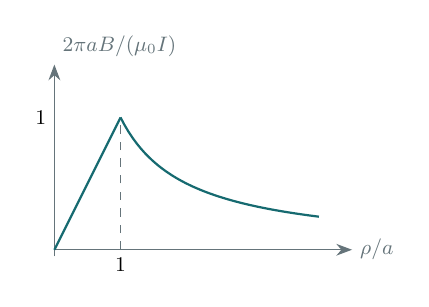
\begin{tikzpicture}[scale=.84,transform shape]
\draw[axis](0,0)--(4.5,0)node[right]{$\rho/a$};\draw[axis](0,-.1)--(0,2.8)node[above right]{$2\pi aB/(\mu_0I)$};\draw[traj](0,0)--(1,2);\draw[traj,domain=1:4,samples=50]plot(\x,{2/\x});\draw[guide](1,0)--(1,2);\node[below]at(1,0){$1$};\node[left]at(0,2){$1$};
\end{tikzpicture}
\figcaption{变图电试1.2V3}
\end{minipage}\end{center}

\Needspace{33\baselineskip}
\item \textbf{题设与求解。}以一组彼此独立的注入平面代替零厚度面，注入位置$s$均匀分布在$[-a,a]$，每个位置的注入电流为$I\,\dd s/(2a)$并在本平面径向分流。所有轴线重合，求层内外总场。图V4中一个位于$s$的单元只在$x<s$贡献无限直导线场，故
\[B_\phi(x,\rho)=\frac{\mu_0I}{2\pi\rho}F(x),\quad
F(x)=\begin{cases}1,&x<-a,\\(a-x)/(2a),&-a\le x\le a,\\0,&x>a.\end{cases}\]
层内方位场线性变化，中面$F(0)=1/2$，层外保持主解两极限。这里明确给出厚度模型：每个平面有自己的轴向供电段和径向分流，而不任意假定只有径向电流、却忽略其连续性所需的轴向电流。$a\to0$时层外趋向阶跃，中面趋向对称平均。
\begin{center}\begin{minipage}{.98\linewidth}\centering
\begin{tikzpicture}[scale=.84,transform shape]
\draw[axis](-2.5,0)--(2.5,0)node[right]{$x/a$};\draw[axis](0,-.2)--(0,2.7)node[above right]{$F$};\draw[traj](-2.2,2)--(-1,2)--(1,0)--(2.2,0);\node[below]at(-1,0){$-1$};\node[below]at(1,0){$1$};\node[left]at(0,1){$1/2$};\node[left]at(0,2){$1$};
\end{tikzpicture}
\figcaption{变图电试1.2V4}
\end{minipage}\end{center}

\Needspace{33\baselineskip}
\item \textbf{题设与求解。}在同一平面设置两个等大反向单元，位于$y=a$的电流为$I$，位于$y=-a$的有向电流为$-I$，$z=0$。求左侧中点磁场及远场。图V5中负电流单元为面内汇流后沿半导线流走，因此电流守恒分别成立。左侧
\[B_z(y,0)=\frac{\mu_0I}{2\pi}\left(\frac1{y-a}-\frac1{y+a}\right)
=\frac{\mu_0I a}{\pi(y^2-a^2)}.\]
中点场为$-\mu_0I/(\pi a)$，两项同向；右侧仍逐套为零。$|y|\gg a$时$B_z\simeq\mu_0I a/(\pi y^2)$，首阶$1/y$项相消。这与两同向单元的远场不同，原因是有向总注入电流为零。图V5以箭头标出两轴旋向，避免把两项的距离当成两个正数后机械相减。
\begin{center}\begin{minipage}{.98\linewidth}\centering
\begin{tikzpicture}[scale=.84,transform shape]
\draw[axis](-2.7,0)--(2.8,0)node[right]{$y$};\node at(-1.5,0){$\otimes$};\node at(1.5,0){$\odot$};\node[below]at(-1.5,-.25){$-I,-a$};\node[below]at(1.5,-.25){$I,a$};\draw[force](0,-.1)--(0,-1.4)node[below]{$\boldsymbol B(P)\parallel-\hat z$};\node[above]at(0,.25){$P$};
\end{tikzpicture}
\figcaption{变图电试1.2V5}
\end{minipage}\end{center}

\Needspace{33\baselineskip}
\item \textbf{题设与求解。}将图V4的均匀注入剖面改为$f(s)=(s+a)/(2a^2)$，$-a<s<a$，每层电流为$If(s)\dd s$。求中面磁场并比较层外总跳变。积分归一为$\int_{-a}^{a}f(s)\dd s=1$，而
\[F(x)=\int_x^a f(s)\dd s=1-\frac{(x+a)^2}{4a^2},\qquad -a\le x\le a.\]
故$B_\phi(0,\rho)=3\mu_0I/(8\pi\rho)$，中面读数对应归一化曲线的$3/4$。图V6的曲线经过$F(0)=3/4$，层外仍从1变到0，跨整层跳变量完全相同。随着$a\to0$，中面值仍由厚度剖面决定；本题零厚度面取对称主值，图V6的非对称剖面则给出另一个确定的中面值。
\begin{center}\begin{minipage}{.98\linewidth}\centering
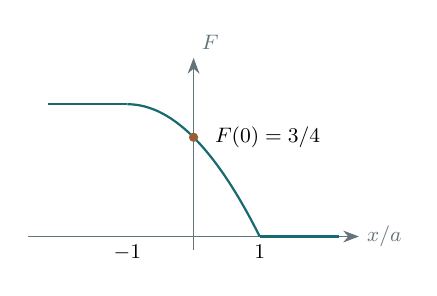
\begin{tikzpicture}[scale=.84,transform shape]
\draw[axis](-2.5,0)--(2.5,0)node[right]{$x/a$};\draw[axis](0,-.2)--(0,2.7)node[above right]{$F$};\draw[traj](-2.2,2)--(-1,2);\draw[traj,domain=-1:1,samples=60]plot(\x,{2*(1-(\x+1)^2/4)});\draw[traj](1,0)--(2.2,0);\fill[warm](0,1.5)circle(2pt);\node[right]at(.2,1.5){$F(0)=3/4$};\node[below]at(-1,0){$-1$};\node[below]at(1,0){$1$};
\end{tikzpicture}
\figcaption{变图电试1.2V6}
\end{minipage}\end{center}

\Needspace{33\baselineskip}
\item \textbf{题设与求解。}在分流面上取$\rho_1<\rho<\rho_2$的完整环形区域。使用对称主值作为作用场，求面电流所受磁力方向与总矢量。图V7中
\[\boldsymbol f_s=\boldsymbol K\times\boldsymbol B_{\rm pv}
=\frac{\mu_0I^2}{8\pi^2\rho^2}\hat x.\]
利用$\hat\rho\times\hat\phi=\hat x$，各处面力都沿$+x$，故积分得
\[\boldsymbol F=\frac{\mu_0I^2}{4\pi}\ln\frac{\rho_2}{\rho_1}\,\hat x.\]
图V7只取远离注入点的有限环域，排除$\rho=0$奇点。由两侧磁应力也得压力$(B_{0^-}^2-B_{0^+}^2)/(2\mu_0)=\mu_0I^2/(8\pi^2\rho^2)$，与平均场方法一致；用左侧全场代替平均场会多一倍。支承和电荷静电力若存在，需另行计入，以上只算磁力。
\begin{center}\begin{minipage}{.98\linewidth}\centering
\begin{tikzpicture}[scale=.84,transform shape]
\fill[accent!12](0,0)circle(1.8);\fill[white](0,0)circle(.8);\draw[object](0,0)circle(1.8);\draw[object](0,0)circle(.8);\draw[guide](0,0)--(1.8,0)node[midway,below]{$\rho_2$};\node at(.35,.65){$\rho_1$};\node at(0,0){$O$};\node[right]at(2.1,.7){环域磁力 $\boldsymbol F\parallel+\hat x$};\node[right]at(2.1,-.4){从 $+x$ 看：$+\hat x$ 指向读者};
\end{tikzpicture}
\figcaption{变图电试1.2V7}
\end{minipage}\end{center}

\Needspace{33\baselineskip}
\item \textbf{题设与求解。}取一个位于分流面左侧、长度为$\ell$、内外半径为$\rho_1,\rho_2$的同轴圆柱壳区域，排除电流轴。求其中磁场能，并比较同样大小的右侧区域。图V8中$\boldsymbol B$在左侧与$x$无关，因而
\[U_L=\int_{\rho_1}^{\rho_2}\frac{B^2}{2\mu_0}\,2\pi\rho\ell\,\dd\rho
=\frac{\mu_0I^2\ell}{4\pi}\ln\frac{\rho_2}{\rho_1},\qquad U_R=0.\]
两个圆柱壳分别完全位于对应半空间内，体积积分只覆盖题设的壳层区域。左侧若令内半径趋零或外半径趋无穷，能量都呈对数发散，表示理想细线与无限范围的局限；有限观察壳内的上式则有限。图V8以阴影标出积分体积，磁场方向沿环向而非沿圆柱轴。
\begin{center}\begin{minipage}{.98\linewidth}\centering
\begin{tikzpicture}[scale=.84,transform shape]
\draw[axis](-3,0)--(3,0)node[right]{$x$};\draw[object](.4,-1.6)--(.4,1.6)node[above]{$x=0$};\fill[accent!10](-2.7,-1.2)rectangle(-.7,1.2);\draw[object](-2.7,-1.2)rectangle(-.7,1.2);\draw[<->,thin,color=muted](-2.7,-1.6)--(-.7,-1.6)node[midway,below]{$\ell$};\node at(-1.7,.55){左壳 $U_L$};\node at(1.8,.55){右壳 $U_R=0$};\node[below]at(.2,-2.4){阴影示子午截面，径向范围 $\rho_1<\rho<\rho_2$};
\end{tikzpicture}
\figcaption{变图电试1.2V8}
\end{minipage}\end{center}
\end{enumerate}

\Needspace{13\baselineskip}

\pdfbookmark[2]{第 3 题 水平磁场中下落带电球的临界轨迹}{q3}

\section*{第 3 题\quad 水平磁场中下落带电球的临界轨迹}\label{q:3}


质量$m$、正电荷$q$的小球在离水平地面高度$h$处由静止开始运动，只受重力和匀强磁场的洛伦兹力。磁场水平，空气阻力、辐射忽略，$g$为常量。
求使小球始终不接触地面的磁感应强度条件，给出临界场值及其轨迹，并说明“严格不接触”时是否存在可取得的最小磁场。
取$x$向右、$y$竖直向下，原点为初始位置，磁场沿$\hat x\times\hat y$方向。


\begin{center}\begin{minipage}{.98\linewidth}\centering
\begin{tikzpicture}[scale=.9,transform shape]

\draw[axis] (0,0)--(5,0) node[right] {$x$};
\draw[axis] (0,0)--(0,-3.7) node[below] {$y$};
\draw[object] (-.5,-3)--(5,-3);
\fill[muted!15] (-.5,-3) rectangle (5,-3.2);
\fill[accent] (0,0) circle (2pt) node[above left] {$O:\ m,q$};
\draw[force] (.4,-.1)--(.4,-1) node[right] {$mg$};
\draw[axis,<->] (4.4,0)--(4.4,-3) node[midway,right] {$h$};
\node at (2.6,-.7) {$\otimes\ \boldsymbol B$};
\node at (2.8,-2.6) {地面 $y=h$};

\end{tikzpicture}
\figcaption{图电试1.3\quad 坐标y向下，磁场指向纸内；初始速度为零。}
\end{minipage}\end{center}

\Needspace{8\baselineskip}

\pdfbookmark[3]{题型定位}{q3-h0}

\subsection*{题型定位}

恒定重力与均匀水平磁场中的带电运动。图A从速度圆确定漂移与回旋，图C把两部分位移合成摆线，图B用最大下落量确定严格不接触条件。求解按动力学、轨迹、接触条件、物理解释的顺序展开。

\Needspace{8\baselineskip}

\pdfbookmark[3]{知识点}{q3-h1}

\subsection*{知识点}

\begin{itemize}
\item 由$q\boldsymbol v\times\boldsymbol B$确定有向分量，回旋角频率为$\omega=qB/m$。
\item 恒定漂移$\boldsymbol v_d$满足$q\boldsymbol v_d\times\boldsymbol B=-m\boldsymbol g$，剩余速度的模保持不变。
\item 相对圆运动与圆心平移给出摆线，空间尺度为$a=g/\omega^2$，时间尺度为$1/\omega$。
\item $2a<h$给严格不接触的开区间，$2a=h$给临界相切；动能由重力做功确定。
\end{itemize}
漂移分解同时确定圆的半径和初相位。由静止释放时回旋速度与漂移等大反向，圆上初点在最高处，因而最大下落量为直径$2a$。改变初速度后，回旋半径和圆上初点随之改变，见变式4—6。

\Needspace{8\baselineskip}

\pdfbookmark[3]{物理图像}{q3-h2}

\subsection*{物理图像}

题图中$y$向下、地面为$y=h$。图A的速度圆经过原点，圆心横坐标为$g/\omega$；图C的空间圆在初始水平线下方，圆心随时间向右平移。图B把临界摆线的最低点与地面画在同一高度，更强磁场给出较小摆线。图D中向上磁力为重力两倍，向上的合力使最低点之后的运动转为上升。

\Needspace{8\baselineskip}

\pdfbookmark[3]{解题入口}{q3-h3}

\subsection*{解题入口}

在题图旁写出磁力分量，初始两分量均为零，因而$\dot v_y(0)=g$。接着从重力与漂移磁力抵消求$v_d$，令$w_x=v_x-v_d$后得到旋转方程。圆的初半径矢量由$\boldsymbol w(0)=-\boldsymbol v_d$确定，随后积分得到位置。判断是否触地时，用$1-\cos\theta$在完整周期内的范围$[0,2]$。

\Needspace{8\baselineskip}

\pdfbookmark[3]{标准解法}{q3-h4}

\subsection*{标准解法}


图电试1.3中地面为$y=h$，磁场垂直运动平面。记
\[
\omega=\frac{qB}{m}>0.
\]
按题图的右手坐标，$\boldsymbol B=B\hat z$、$\boldsymbol g=g\hat y$，速度始终在$xy$平面内。由叉乘直接得到
\[
q\boldsymbol v\times\boldsymbol B=qB(v_y\hat x-v_x\hat y).
\]
因此向下速度产生向右磁力，向右速度产生向上磁力。初始速度为零时磁力也为零，竖直初加速度为$g$。洛伦兹力分量给
\[
\dot v_x=\omega v_y,\qquad
\dot v_y=g-\omega v_x,\qquad v_x(0)=v_y(0)=0.
\]
选取恒定水平速度，使它的磁力抵消重力，可将含$g$的方程化为纯旋转方程。这给出
\[
q\boldsymbol v_d\times\boldsymbol B=-mg\hat y,
\qquad v_d=\frac{mg}{qB}=\frac g\omega.
\]
把速度分为这项常量漂移和相对速度：
\[
\boldsymbol v=\boldsymbol v_d+\boldsymbol w,\qquad
\boldsymbol v_d=\frac g\omega\hat x.
\]
漂移速度的磁力恰向上抵消重力，故
\[
\dot w_x=\omega w_y,\qquad \dot w_y=-\omega w_x,
\quad
\boldsymbol w(0)=-\frac g\omega\hat x.
\]
\begin{center}\begin{minipage}{.98\linewidth}\centering
\begin{tikzpicture}[scale=.85,transform shape]

\draw[axis] (0,0)--(4,0) node[right] {$v_x$};
\draw[axis] (0,1.9)--(0,-2) node[below] {$v_y$};
\draw[object] (1.5,0) circle (1.5);
\draw[motion] (0,0)--(1.5,0) node[midway,above] {$\boldsymbol v_d$};
\draw[motion] (1.5,0)--(.75,-1.299) node[midway,right] {$\boldsymbol w$};
\draw[force] (0,0)--(.75,-1.299);
\draw[guide] (.375,-.65)--(-.45,-.8);
\node[left] at (-.45,-.8) {$\boldsymbol v$};
\fill (1.5,0) circle (1.5pt) node[above right] {$g/\omega$};
\node at (2.2,2.1) {$|\boldsymbol w|=g/\omega$};
\node[above left] at (0,0) {初态};

\end{tikzpicture}
\figcaption{解图电试1.3A\quad 实际速度是漂移速度与旋转速度相加，速度圆经过零点。}
\end{minipage}\end{center}
在以$\boldsymbol v_d$平移的参考系中，重力与漂移所对应的那部分磁力抵消，剩余合力为$q\boldsymbol w\times\boldsymbol B$。该力随$\boldsymbol w$转向，始终垂直$\boldsymbol w$，因此相对速度的大小保持不变，方向连续旋转。回旋角速度由力与相对速度之比确定，为$qB/m$；相对速度转过一周所需时间为$2\pi/\omega$。这就把恒定重力作用下的运动化成了一个圆心匀速平移、半径保持不变的运动。

解图电试1.3A中的速度圆以$\boldsymbol v_d$为圆心。由旋转方程，
\[
\frac{\dd}{\dd t}(w_x^2+w_y^2)
=2w_x\omega w_y-2w_y\omega w_x=0,
\qquad |\boldsymbol w|=\frac g\omega.
\]
相对速度的初始方向向左，随后转向下方。对$w_x$再求导，得$\ddot w_x+\omega^2w_x=0$；以$w_x(0)=-g/\omega,\dot w_x(0)=0$确定余弦项，并由$w_y=\dot w_x/\omega$求得正弦项。加上向右的$\boldsymbol v_d$，实际速度为：
\[
\boxed{v_x=\frac g\omega(1-\cos\omega t),\qquad
v_y=\frac g\omega\sin\omega t}.
\]
分别对两速度分量积分，水平方向的常量项给$(g/\omega)t$，余弦项给$-(g/\omega^2)\sin\omega t$；竖直方向给$-(g/\omega^2)\cos\omega t$及积分常量$g/\omega^2$。用$x(0)=y(0)=0$得到
\[
\boxed{x=a(\omega t-\sin\omega t),\qquad
y=a(1-\cos\omega t)},\qquad
a=\frac g{\omega^2}=\frac{m^2g}{q^2B^2}.
\]
解图C给出轨迹的几何合成。令$\theta=\omega t$，滚圆圆心为$C=(a\theta,a)$，圆上一点相对圆心的坐标为$(-a\sin\theta,-a\cos\theta)$。圆心以$a\omega=g/\omega$向右平移，半径矢量以角速度$\omega$转动；两个坐标相加正好是上式。圆的半径$a=m v_d/(qB)$同时等于相对回旋半径。初始点位于圆的最高点，相对速度向左与圆心速度相消，满足由静止释放的初态。

\begin{center}\begin{minipage}{.98\linewidth}\centering
\begin{tikzpicture}[scale=.86,transform shape]

\draw[axis](-.5,0)--(5,0)node[right]{$x$};\draw[axis](0,.3)--(0,-2.9)node[below]{$y$};
\draw[object](1.5708,-1)circle(1);\fill[accent](1.5708,-1)circle(2pt)node[right]{$C=(a\theta,a)$};
\fill[warm](.5708,-1)circle(2pt)node[left]{$P$};\draw[guide](1.5708,-1)--(.5708,-1)node[midway,below]{$a$};
\draw[motion](1.5708,-.75)--(3,-.75)node[right]{$v_d=a\omega$};\draw[motion](.5708,-1.15)--(.5708,-1.9)node[below]{$\boldsymbol w$};
\draw[guide](1.5708,-1)--(1.5708,0);\node[above]at(1.5708,0){圆心上方切点};\node[below]at(2.5,-2.6){图示 $\theta=\pi/2$，圆沿顶部水平线滚动};

\end{tikzpicture}
\figcaption{解图电试1.3C\quad 平移圆心与旋转半径共同生成摆线}
\end{minipage}\end{center}
摆线的$y$最大值为$2a$，首次发生在$\omega t=\pi$；该时刻竖直速度为零，水平方向仍有速度$2g/\omega$。
\begin{center}\begin{minipage}{.98\linewidth}\centering
\begin{tikzpicture}[scale=.85,transform shape]

\draw[axis] (0,0)--(7,0) node[right] {$x$};
\draw[axis] (0,0)--(0,-2.9) node[below] {$y$};
\draw[object] (-.3,-2)--(6.8,-2);
\draw[traj,domain=0:6.283185,samples=110] plot ({\x-sin(deg(\x))},{-1+cos(deg(\x))});
\draw[thick,dashed,color=warm,domain=0:6.283185,samples=110] plot ({.75*(\x-sin(deg(\x)))},{-.75*(1-cos(deg(\x)))});
\fill (3.14159,-2) circle (1.6pt) node[below] {临界接触};
\node[above,color=accent] at (5,-.8) {$B=B_*$};
\node[above,color=warm] at (2,-1.2) {$B>B_*$};
\node[right] at (6.8,-2) {$y=h$};
\draw[axis,<->] (6.5,0)--(6.5,-2) node[midway,right] {$h=2a_*$};
\node[below] at (0,0) {$O$};

\end{tikzpicture}
\figcaption{解图电试1.3B\quad 临界摆线相切地面；更强磁场的虚线轨迹仍留间隙。}
\end{minipage}\end{center}
沿图B的第一段轨迹观察，$0<\theta<\pi$时$\sin\theta>0$，所以竖直速度向下；$\pi<\theta<2\pi$时竖直速度向上。四分之一周期时，$x=a(\pi/2-1),y=a$，两速度分量同为$g/\omega$，切线向右下方；半周期时下落到$2a$，切线转为水平。后半周期回升到初始高度，水平方向仍在前进，于是相邻两个零速度尖点之间构成一个完整摆线拱。

固定$m,q,g$而增强磁场，时间尺度$1/\omega$按$1/B$减小，空间尺度$a$按$1/B^2$减小，速度尺度$g/\omega$按$1/B$减小。因而小球更早转入上升段，最大下落量也更小。图B中虚线摆线的高度和每个拱的水平宽度同时缩小，地面位置则由给定的$h$保持不变。判定场强时，正是比较这个随场变化的最大下落量与固定地面高度。

解图电试1.3B把地面画在初始水平线下$h$处。严格不接触要求摆线最低点仍在地面上方，即
\[
2a<h
\quad\Longleftrightarrow\quad
\boxed{B>B_*},\qquad
\boxed{B_*=\frac m q\sqrt{\frac{2g}{h}}}.
\]
在$B=B_*$时，$a=h/2$，临界轨迹为
\[
x=\frac h2(\theta-\sin\theta),\qquad
y=\frac h2(1-\cos\theta),\qquad
\theta=\sqrt{\frac{2g}{h}}\,t.
\]
它在$\theta=(2k+1)\pi$处与地面相切。严格不接触的允许区间是$(B_*,\infty)$，下确界为$B_*$，这个开区间没有可取得的最小场强。等号$B=B_*$描述恰好相切的临界轨迹。

若$0<B<B_*$，第一段下降过程便有$y=h$。由
\[
\cos\theta_c=1-\frac h a,\qquad 0<\theta_c<\pi
\]
可知首次到达地面时小球仍有向下速度，摆线描述从释放到首次接触的这一段运动。具体地，首次接触时刻和水平位置为
\[
t_c=\frac{\theta_c}{\omega},\qquad
x_c=a(\theta_c-\sin\theta_c).
\]
用接触条件$1-\cos\theta_c=h/a$代入速度式，可直接得到
\[
v_{x,c}=\omega h,\qquad
v_{y,c}=\sqrt{2gh-\omega^2h^2}>0.
\]
这两个分量给出到达地面时的方向：场越接近临界值，竖直分量越小、切线越接近水平；在临界等号处，竖直分量为零而水平分量达到$\sqrt{2gh}$。当$B$趋于零，接触时间趋于$\sqrt{2h/g}$，水平分量趋零，竖直分量趋于$\sqrt{2gh}$，连续接到自由落体。$B=0$时直接由$y=gt^2/2$描述下落。

\textbf{最低点的受力与动能变化。}在$\theta=\pi$，$v_y=0$、$v_x=2g/\omega$，向上磁力为$qB(2g/\omega)=2mg$，重力向下为$mg$，所以净加速度向上为$g$。图D的速度箭头水平向右，合力箭头向上，随后小球进入上升段。这个转折由竖直速度的变号确定。

\begin{center}\begin{minipage}{.98\linewidth}\centering
\begin{tikzpicture}[scale=.86,transform shape]

\draw[axis](-1,0)--(4,0)node[right]{$x$};\fill[accent](0,0)circle(3pt)node[below left]{最低点};
\draw[motion](0,.2)--(2.8,.2)node[right]{$v_x=2g/\omega$};
\draw[force](0,.35)--(0,2.35)node[above]{$F_B=2mg$};\draw[force](.3,-.15)--(.3,-1.15)node[below]{$mg$};
\draw[motion](2,-.4)--(2,.6)node[right]{$\boldsymbol a=-g\hat y$};\node[below]at(1.3,-1.9){竖直速度为零时，向上的合力使轨迹转弯};

\end{tikzpicture}
\figcaption{解图电试1.3D\quad 最低点的速度、磁力与重力}
\end{minipage}\end{center}
沿运动方程与速度作点积，磁力项为零，得$m\boldsymbol v\cdot\dot{\boldsymbol v}=mgv_y$。从初态积分即有$mv^2/2=mgy$。把速度分量写入这个能量关系：
\[
v^2=\frac{g^2}{\omega^2}
[(1-\cos\theta)^2+\sin^2\theta]
=2ga(1-\cos\theta)=2gy.
\]
每到$\theta=2k\pi$，位置回到初始高度、速度也再次为零，形成摆线尖点。每个周期水平方向前进$2\pi a$；相对回旋速度恒定，而地面系速率随重力做功周期变化。


\Needspace{8\baselineskip}

\pdfbookmark[3]{关键洞察}{q3-h5}

\subsection*{关键洞察}

速度的圆心平移量在速度空间是常量，在位置空间则积累为水平匀速漂移。最低点具有水平速度$2g/\omega$，竖直加速度向上；初始点和每周期尖点的速度则为零，竖直加速度向下。接触由整条轨迹的最大下落量决定，严格条件的下确界对应临界相切。

\Needspace{8\baselineskip}

\pdfbookmark[3]{易错点}{q3-h6}

\subsection*{易错点}

\begin{itemize}
\item 最低点由$v_y=0$确定，该点磁力为$2mg$、合力向上为$mg$。
\item 地面轨迹包括圆心平移和相对圆周运动两项，实际速率随时间变化。
\item 严格不接触使用$2a<h$，临界图使用$2a=h$，两种取值在图B中分别标出。
\item 当$2a>h$时，运动段终止于首次触地，时刻由$\cos\theta_c=1-h/a$求出。
\item 磁力始终不做功，重力改变动能，整个自由运动段满足$v^2=2gy$。
\end{itemize}

\Needspace{8\baselineskip}

\pdfbookmark[3]{课堂讲解建议}{q3-h7}

\subsection*{课堂讲解建议}

让学生用右手规则给题图中的向下速度画磁力，再从分量方程求出漂移速度。在图A上从零速度出发标出四分之一周期与半周期的位置，依次得到速度和轨迹。画出图C后，要求说明圆心为什么每转一周前进一个周长。到最低点时，让学生在图D上标出速度、重力、磁力和合力，并用向上的合力解释随后的上升。最后把地面分别放在$h>2a,h=2a,h<2a$三处，讨论不接触、相切、首次碰撞三个具体过程。

\Needspace{8\baselineskip}

\pdfbookmark[3]{变式训练}{q3-h8}

\subsection*{变式训练}

\begin{enumerate}
\Needspace{33\baselineskip}
\item 只要求从释放起到$t_f$的有限时段内严格不触地，求条件，并给出有限时安全而完整周期会触地的例子。
\textbf{解：}图V1把观测时段标在第一段下降过程中。记$\theta_f=\omega t_f$，若$0\le\theta_f\le\pi$，$y$单调增大，最大值为$a(1-\cos\theta_f)$；若$\theta_f\ge\pi$，时段已经包含第一次最低点，最大值为$2a$。因此
\[\max y=\begin{cases}a(1-\cos\theta_f),&\theta_f\le\pi,\\2a,&\theta_f\ge\pi,\end{cases}\qquad \max y<h.\]
例如$a=0.8h,\theta_f=\pi/2$时，时段终点只下落$0.8h$；继续运动将在$\theta_c=\arccos(-1/4)$首次触地。这说明有限观测时间与完整周期对应不同的最大值区间。
\begin{center}\begin{minipage}{.98\linewidth}\centering
\begin{tikzpicture}[scale=.86,transform shape]
\draw[axis](0,0)--(3.5,0)node[right]{$\theta/\pi$};\draw[axis](0,.2)--(0,-2.5)node[below]{$y/h$};\draw[traj,domain=0:pi,samples=60]plot({\x/pi*3},{-.8*(1-cos(deg(\x)))});\draw[object](-.1,-1)--(3.3,-1)node[right]{地面};\draw[guide](1.5,0)--(1.5,-.8);\node[above]at(1.5,0){$t_f$};\node[below]at(3,0){$1$};
\end{tikzpicture}
\figcaption{变图电试1.3V1}
\end{minipage}\end{center}

\Needspace{33\baselineskip}
\item 将电荷改为$-q$而保持磁场方向及初态，求轨迹与场强条件。
\textbf{解：}图V2以相同向下坐标比较两个电荷符号。用有向$\omega_s=-qB/m$写速度和位置，
\[v_x=\frac g{\omega_s}(1-\cos\omega_st),\quad v_y=\frac g{\omega_s}\sin\omega_st,\quad
x=\frac g{\omega_s^2}(\omega_st-\sin\omega_st),\quad y=\frac g{\omega_s^2}(1-\cos\omega_st).\]
$x$反号而$y$保持不变，两条摆线关于竖直轴镜像。最大下落仍为$2m^2g/(q^2B^2)$，严格不触地条件使用电荷绝对值$B>(m/|q|)\sqrt{2g/h}$。正电荷向右漂移，负电荷向左漂移，二者的重力做功和动能变化相同。
\begin{center}\begin{minipage}{.98\linewidth}\centering
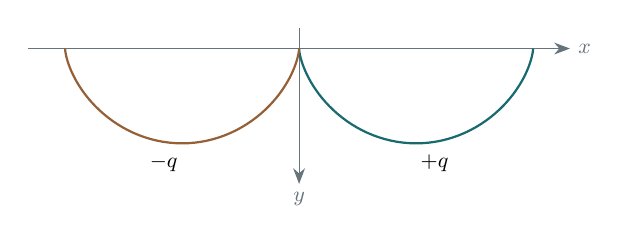
\begin{tikzpicture}[scale=.86,transform shape]
\draw[axis](-4,0)--(4,0)node[right]{$x$};\draw[axis](0,.3)--(0,-2)node[below]{$y$};\draw[traj,domain=0:2*pi,samples=75]plot({.55*(\x-sin(deg(\x)))},{-.7*(1-cos(deg(\x)))});\draw[thick,color=warm,domain=0:2*pi,samples=75]plot({-.55*(\x-sin(deg(\x)))},{-.7*(1-cos(deg(\x)))});\node at(2,-1.7){$+q$};\node at(-2,-1.7){$-q$};
\end{tikzpicture}
\figcaption{变图电试1.3V2}
\end{minipage}\end{center}

\Needspace{33\baselineskip}
\item 磁场取临界值，求第一次与地面相切的时刻、水平位置、速率及该处磁力。
\textbf{解：}图V3的相切点对应$\theta=\pi,a=h/2,\omega=\sqrt{2g/h}$，故
\[t_c=\pi\sqrt{\frac h{2g}},\qquad x_c=\frac{\pi h}{2},\qquad v_c=\frac{2g}{\omega}=\sqrt{2gh}.\]
向上磁力$qB_*v_c=2mg$，重力向下为$mg$，净加速度向上为$g$。由$v_c^2=2gh$也可读出下落高度$h$所增加的动能。此处竖直速度为零、水平速度沿地面，轨迹的切线与地面平行；几何上已发生接触，严格不触地的场强位于临界值以上。
\begin{center}\begin{minipage}{.98\linewidth}\centering
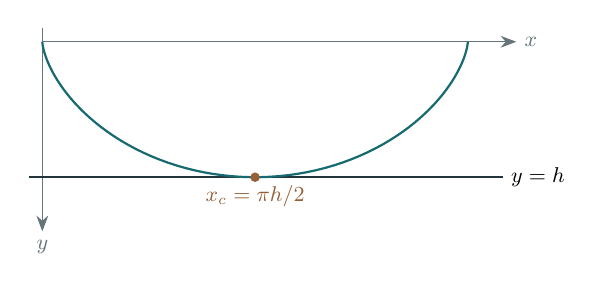
\begin{tikzpicture}[scale=.86,transform shape]
\draw[axis](0,0)--(7,0)node[right]{$x$};\draw[axis](0,.2)--(0,-2.8)node[below]{$y$};\draw[object](-.2,-2)--(6.8,-2);\draw[traj,domain=0:2*pi,samples=90]plot({\x-sin(deg(\x))},{-(1-cos(deg(\x)))});\fill[warm](pi,-2)circle(2pt)node[below]{$x_c=\pi h/2$};\node[right]at(6.8,-2){$y=h$};
\end{tikzpicture}
\figcaption{变图电试1.3V3}
\end{minipage}\end{center}

\Needspace{33\baselineskip}
\item 初速度取向右的$v_d=g/\omega$，其余条件保持，求运动；再比较由静止释放。
\textbf{解：}图V4中初始相对速度$\boldsymbol w(0)=0$。旋转方程使$\boldsymbol w(t)$始终为零，于是
\[v_x=v_d,\quad v_y=0,\quad x=v_dt,\quad y=0.\]
重力与漂移磁力在每个时刻抵消，小球沿初始高度水平匀速运动。由静止释放时则有$\boldsymbol w(0)=-v_d\hat x$，产生半径$a$的相对圆运动，最大下落$2a$。同一外场下，轨迹的回旋幅度由初速度相对漂移速度的差确定。
\begin{center}\begin{minipage}{.98\linewidth}\centering
\begin{tikzpicture}[scale=.86,transform shape]
\draw[axis](0,0)--(5.2,0)node[right]{$x$};\draw[axis](0,.2)--(0,-2.7)node[below]{$y$};\draw[traj](0,0)--(4.8,0);\draw[motion](1,.25)--(3,.25)node[midway,above]{$v_d$};\draw[thick,dashed,color=warm,domain=0:2*pi,samples=80]plot({.7*(\x-sin(deg(\x)))},{-(1-cos(deg(\x)))});\node[below]at(2.4,-2.2){虚线：由静止释放};
\end{tikzpicture}
\figcaption{变图电试1.3V4}
\end{minipage}\end{center}

\Needspace{33\baselineskip}
\item 初速度沿水平方向，大小为有向$u_0$，竖直初速为零。求最大下落量及不触地条件。
\textbf{解：}令$\alpha=u_0/v_d$。由相对速度初值$w_x(0)=u_0-v_d,w_y(0)=0$，
\[x=v_dt+\frac{u_0-v_d}{\omega}\sin\omega t,\qquad
y=a(1-\alpha)(1-\cos\omega t).\]
图V5画$\alpha=0,1/2,1,3/2$时的竖直位移。$\alpha<1$时最大下落为$2a(1-\alpha)$，严格不触地要求它小于$h$；$\alpha\ge1$时$y\le0$，小球始终位于初始高度或其上方。$\alpha=1$恢复水平匀速轨迹；负$u_0$则增大向下摆幅。
\begin{center}\begin{minipage}{.98\linewidth}\centering
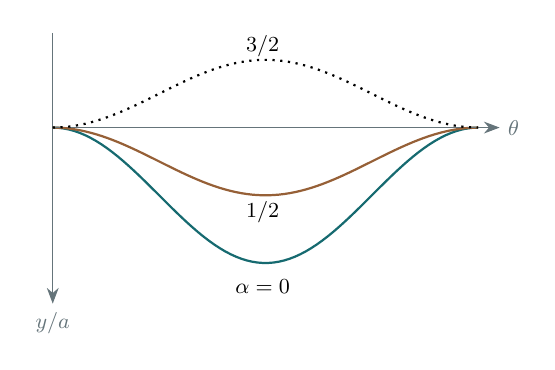
\begin{tikzpicture}[scale=.86,transform shape]
\draw[axis](0,0)--(6.6,0)node[right]{$\theta$};\draw[axis](0,1.4)--(0,-2.6)node[below]{$y/a$};\draw[traj,domain=0:2*pi,samples=80]plot(\x,{-(1-cos(deg(\x)))});\draw[thick,color=warm,domain=0:2*pi,samples=80]plot(\x,{-.5*(1-cos(deg(\x)))});\draw[guide](0,0)--(6.28,0);\draw[thick,dotted,domain=0:2*pi,samples=80]plot(\x,{.5*(1-cos(deg(\x)))});\node at(3.1,-2.35){$\alpha=0$};\node at(3.1,-1.25){$1/2$};\node at(3.1,1.2){$3/2$};
\end{tikzpicture}
\figcaption{变图电试1.3V5}
\end{minipage}\end{center}

\Needspace{33\baselineskip}
\item 释放时另有竖直向下初速度$v_0>0$，水平初速为零，求最大下落量及严格不触地场强。
\textbf{解：}图V6中速度圆仍以$v_d\hat x$为圆心，半径变为$\sqrt{v_d^2+v_0^2}$。积分得
\[y=a(1-\cos\theta)+\frac{v_0}{\omega}\sin\theta,\quad
x=a(\theta-\sin\theta)+\frac{v_0}{\omega}(1-\cos\theta).\]
将$-a\cos\theta+(v_0/\omega)\sin\theta$合成为一个正弦，得到$y_{\max}=a+\sqrt{a^2+(v_0/\omega)^2}$。要求$h>y_{\max}$，移项平方后化为
\[\omega^2h^2>2gh+v_0^2,\qquad
B>\frac mq\sqrt{\frac{2g}{h}+\frac{v_0^2}{h^2}}.\]
第一次最低点在$\theta=\pi-\arctan(v_0/v_d)$，比静止释放更早到达；$v_0\to0$时恢复主解。
\begin{center}\begin{minipage}{.98\linewidth}\centering
\begin{tikzpicture}[scale=.86,transform shape]
\draw[axis](-.5,0)--(4,0)node[right]{$v_x$};\draw[axis](0,2)--(0,-2.2)node[below]{$v_y$};\draw[object](1.4,0)circle(1.72);\fill[warm](0,-1)circle(2pt)node[below left]{初速度 $v_0$};\fill[accent](1.4,0)circle(2pt)node[above right]{$v_d$};\draw[guide](1.4,0)--(0,-1);\node at(2,-2){半径 $\sqrt{v_d^2+v_0^2}$};
\end{tikzpicture}
\figcaption{变图电试1.3V6}
\end{minipage}\end{center}

\Needspace{33\baselineskip}
\item 磁场与向下竖直方向夹角为$\beta$，$0<\beta\le\pi/2$，其余仍由静止释放。讨论是否能用有限场强始终避开无限大水平地面。
\textbf{解：}图V7把重力分成沿场的$g\cos\beta$和垂直场的$g\sin\beta$。沿场分量产生匀加速运动，垂直场分量产生漂移与回旋。漂移方向水平，其竖直位移为零，合成竖直下落为
\[y(t)=\frac12g\cos^2\beta\,t^2+
\frac{g\sin^2\beta}{\omega^2}(1-\cos\omega t).\]
当$\cos\beta\ne0$，第一项随$t^2$增长而第二项非负，所以任意有限$B$最终都会到达$y=h$。水平磁场$\beta=\pi/2$使沿场重力消失，竖直下落才保持有界并恢复$2g/\omega^2<h$。
\begin{center}\begin{minipage}{.98\linewidth}\centering
\begin{tikzpicture}[scale=.86,transform shape]
\draw[axis](0,1)--(0,-3)node[below]{$\hat y$};\draw[axis](-1,0)--(4,0);\draw[motion](0,0)--(2.2,-1.8)node[right]{$\boldsymbol B$};\draw[force](0,0)--(0,-2)node[below left]{$m\boldsymbol g$};\draw[guide](0,-2)--(1,-.82);\draw[force](0,0)--(1,-.82)node[midway,above right]{$mg\cos\beta$};\node[left]at(-.15,-.6){$\beta$};\node[below]at(1.4,-3.4){沿场重力给出无界的竖直下落};
\end{tikzpicture}
\figcaption{变图电试1.3V7}
\end{minipage}\end{center}

\Needspace{33\baselineskip}
\item 由静止释放的轨迹测得相邻尖点时间间隔$T$、水平间隔$P$，已知磁场$B$，求质量电荷比，并给出最大下落量与$P,T,g$的关系。
\textbf{解：}图V8中每个周期圆心前进一个周长，故
\[T=\frac{2\pi}{\omega},\quad P=2\pi a,\quad
\frac mq=\frac{BT}{2\pi},\qquad d_{\max}=2a=\frac P\pi.\]
结合$a=g/\omega^2$，又有$P=gT^2/(2\pi)$，因此$g=2\pi P/T^2$。时间尺度给出回旋频率，空间尺度给出漂移速度$P/T$；两项数据共同描述同一条由静止释放的摆线。已知$g$时，测量应满足上述关系，严格不触地可直接写为$P<\pi h$。
\begin{center}\begin{minipage}{.98\linewidth}\centering
\begin{tikzpicture}[scale=.86,transform shape]
\draw[axis](0,0)--(7.5,0)node[right]{$x$};\draw[traj,domain=0:4*pi,samples=120]plot({.55*(\x-sin(deg(\x)))},{-.8*(1-cos(deg(\x)))});\draw[<->,thin,color=muted](0,.6)--(3.45575,.6)node[midway,above]{$P$，历时 $T$};\draw[<->,thin,color=muted](3.8,0)--(3.8,-1.6)node[midway,right]{$d_{\max}=P/\pi$};
\end{tikzpicture}
\figcaption{变图电试1.3V8}
\end{minipage}\end{center}
\end{enumerate}

\Needspace{13\baselineskip}

\pdfbookmark[2]{第 4 题 弱磁场中异号带电双体的质心摆线}{q4}

\section*{第 4 题\quad 弱磁场中异号带电双体的质心摆线}\label{q:4}


质量均为$m$、电荷分别为$+q$与$-q$的两质点相距$2R$。以其质心$C$为原点，取$x$向右、$y$向上。$t=0$时$+q$在$(0,-R)$、$-q$在$(0,R)$，两者速度构成绕$C$顺时针的半径$R$圆运动，质心初速为零。初始圆运动角频率$\omega$由库仑引力确定。
考察这一初态在沿$+z$的弱匀强静磁场$\boldsymbol B=B\hat z$中的后续运动；忽略重力、辐射及建场过程的感应冲量。取$qB/(m\omega)\ll1$，只求关于$B$的一阶质心运动，近似保持内部圆运动不变。
\begin{enumerate}
\item 求$v_{Cx}(t),v_{Cy}(t)$。
\item 求$X_C(t),Y_C(t)$并画轨迹。
\item 说明这一近似为何不与磁力不做功、系统能量守恒矛盾。
\end{enumerate}


\begin{center}\begin{minipage}{.98\linewidth}\centering
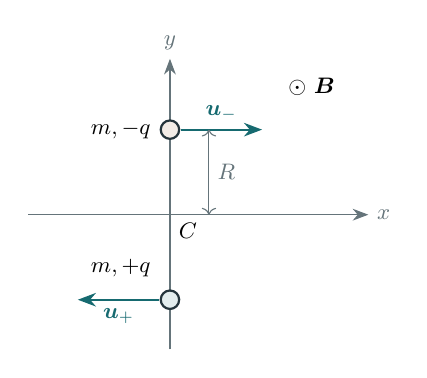
\begin{tikzpicture}[scale=.9,transform shape]

\draw[axis] (-2,0)--(2.8,0) node[right] {$x$};
\draw[axis] (0,-1.9)--(0,2.2) node[above] {$y$};
\fill[accent!12] (0,-1.2) circle (.13);\draw[object] (0,-1.2) circle (.13);
\fill[warm!12] (0,1.2) circle (.13);\draw[object] (0,1.2) circle (.13);
\node[left] at (-.15,1.2) {$m,-q$};\node[above left] at (-.15,-1) {$m,+q$};
\draw[motion] (.15,1.2)--(1.3,1.2) node[midway,above] {$\boldsymbol u_-$};
\draw[motion] (-.15,-1.2)--(-1.3,-1.2) node[midway,below] {$\boldsymbol u_+$};
\node[below right] at (0,0) {$C$};
\node at (2,1.8) {$\odot\ \boldsymbol B$};
\draw[axis,<->] (.55,0)--(.55,1.2) node[midway,right] {$R$};

\end{tikzpicture}
\figcaption{图电试1.4\quad 上方负电荷向右、下方正电荷向左，初始内部运动顺时针。}
\end{minipage}\end{center}

\Needspace{8\baselineskip}

\pdfbookmark[3]{题型定位}{q4-h0}

\subsection*{题型定位}

中性双体的内部转动在均匀磁场中产生旋转的合外力。先从库仑圆运动求$\omega$，按两电荷的完整速度求总磁力，再连续积分得到质心摆线。最后由相对方程和功率分解说明一阶位移与二阶能量的关系。

\Needspace{8\baselineskip}

\pdfbookmark[3]{知识点}{q4-h1}

\subsection*{知识点}

\begin{itemize}
\item 库仑力在初态提供圆周运动的向心力，$\omega^2=q^2/(16\pi\varepsilon_0mR^3)$。
\item 速度分成质心速度与内部速度，求磁力时分别乘带符号电荷。
\item 总力中共同平移项相消，反向内部速度与异号电荷使两内部磁力相加。
\item 旋转总力两次积分含非零常量项，该项确定摆线漂移和初始零速。
\item 位移从$O(B)$出现、质心动能从$O(B^2)$出现，内部反馈按相同阶次处理。
\end{itemize}
精确的质心速度与内部位移关系把外力积分与几何构型相连；等质量和零质心初速共同使内部轨道的磁反馈从二阶进入。

\Needspace{8\baselineskip}

\pdfbookmark[3]{物理图像}{q4-h2}

\subsection*{物理图像}

题图中上方负电荷向右、下方正电荷向左，两磁力均向上。图A把两项磁力与总力的起始方向画在一起。图B中平移与圆周运动速度尺度相同，初始相消形成尖点，半周期则同向相加。图C比较内部半径$R$与质心滚圆半径$\epsilon R$。图D用同一能量单位画质心增能与内部减能，两曲线在每一时刻取相反值。

\Needspace{8\baselineskip}

\pdfbookmark[3]{解题入口}{q4-h3}

\subsection*{解题入口}

先在题图写正电荷的内部位置和速度，再将负电荷取反。对两个地面速度分别作叉乘后相加，共同速度项自动消失。将旋转总力除以总质量$2m$，每次积分都从0到$t$写出上下限，依次确定质心速度与位置。图B的圆分解随后解释为什么轨迹具有漂移和周期尖点。

\Needspace{8\baselineskip}

\pdfbookmark[3]{标准解法}{q4-h4}

\subsection*{标准解法}


图电试1.4中$+q$在下方，顺时针运动使它的初速度向左。未受磁场扰动的库仑圆运动满足
\[
m\omega^2R=\frac{q^2}{4\pi\varepsilon_0(2R)^2},
\qquad
\boxed{\omega=\frac{q}{4R\sqrt{\pi\varepsilon_0mR}}}.
\]
以零阶内部圆运动作为一阶磁力计算中的速度，
\[
\boldsymbol r_+=(-R\sin\omega t,-R\cos\omega t),\qquad
\boldsymbol r_-=-\boldsymbol r_+,
\]
\[
\boldsymbol u_+=(-\omega R\cos\omega t,\ \omega R\sin\omega t),
\qquad \boldsymbol u_-=-\boldsymbol u_+.
\]
两个粒子的地面速度分别为$\boldsymbol V_C+\boldsymbol u_+$和$\boldsymbol V_C-\boldsymbol u_+$。它们的磁力之和为
\[
\boldsymbol F_{\rm ext}
=q(\boldsymbol V_C+\boldsymbol u_+)\times\boldsymbol B
-q(\boldsymbol V_C-\boldsymbol u_+)\times\boldsymbol B
=2q\boldsymbol u_+\times\boldsymbol B.
\]
质心速度所致的两项在总力中严格相消，内部库仑力也相消。
\begin{center}\begin{minipage}{.98\linewidth}\centering
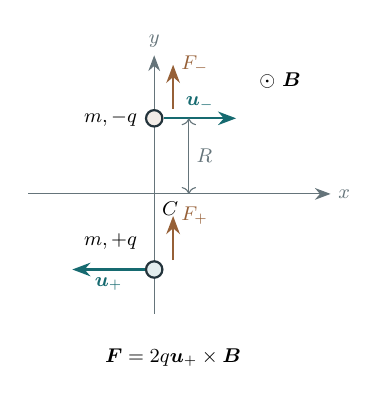
\begin{tikzpicture}[scale=.8,transform shape]

\draw[axis] (-2,0)--(2.8,0) node[right] {$x$};
\draw[axis] (0,-1.9)--(0,2.2) node[above] {$y$};
\fill[accent!12] (0,-1.2) circle (.13);\draw[object] (0,-1.2) circle (.13);
\fill[warm!12] (0,1.2) circle (.13);\draw[object] (0,1.2) circle (.13);
\node[left] at (-.15,1.2) {$m,-q$};\node[above left] at (-.15,-1) {$m,+q$};
\draw[motion] (.15,1.2)--(1.3,1.2) node[midway,above] {$\boldsymbol u_-$};
\draw[motion] (-.15,-1.2)--(-1.3,-1.2) node[midway,below] {$\boldsymbol u_+$};
\node[below right] at (0,0) {$C$};
\node at (2,1.8) {$\odot\ \boldsymbol B$};
\draw[axis,<->] (.55,0)--(.55,1.2) node[midway,right] {$R$};

\draw[force] (.3,1.35)--(.3,2.05) node[right] {$F_-$};
\draw[force] (.3,-1.05)--(.3,-.35) node[right] {$F_+$};
\node at (.3,-2.6) {$\boldsymbol F=2q\boldsymbol u_+\times\boldsymbol B$};

\end{tikzpicture}
\figcaption{解图电试1.4A\quad 异号电荷的内部速度反向，两磁力却同向，初始总力向上。}
\end{minipage}\end{center}
解图电试1.4A中$t=0$两磁力均向$+y$。任意时刻总力分量为
\[
F_x=2q\omega RB\sin\omega t,\qquad
F_y=2q\omega RB\cos\omega t.
\]
总质量为$2m$，故$\dot v_{Cx}=(q\omega RB/m)\sin\omega t$、$\dot v_{Cy}=(q\omega RB/m)\cos\omega t$。从0到$t$积分时，正弦项给$(1-\cos\omega t)/\omega$，余弦项给$\sin\omega t/\omega$。取$\boldsymbol V_C(0)=0$，得
\[
\boxed{v_{Cx}=\frac{qBR}{m}(1-\cos\omega t),\qquad
v_{Cy}=\frac{qBR}{m}\sin\omega t}.
\]
水平方向速度含常量$qBR/m$及余弦项，竖直方向速度为正弦项。分别积分，前者产生匀速平移和正弦位移，后者产生余弦位移。再用$X_C(0)=Y_C(0)=0$确定常数，得到
\[
\boxed{X_C=A(\omega t-\sin\omega t),\qquad
Y_C=A(1-\cos\omega t)},\qquad
A=\frac{qBR}{m\omega}.
\]
代入$\omega$可写
\[
A=4BR^2\sqrt{\frac{\pi\varepsilon_0R}{m}}.
\]
\begin{center}\begin{minipage}{.98\linewidth}\centering
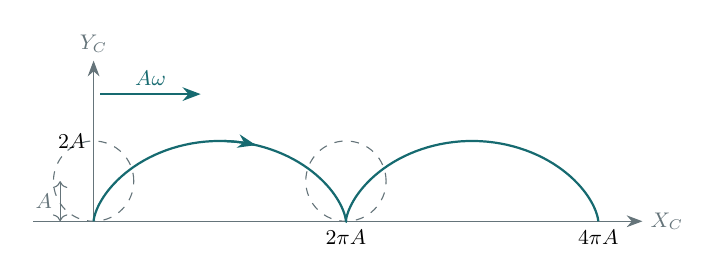
\begin{tikzpicture}[scale=.85,transform shape]

\draw[axis] (-.9,0)--(8.2,0) node[right] {$X_C$};
\draw[axis] (0,0)--(0,2.4) node[above] {$Y_C$};
\draw[guide] (0,.6) circle (.6);
\draw[guide] (3.76991,.6) circle (.6);
\draw[traj,domain=0:12.56637,samples=150] plot ({.6*(\x-sin(deg(\x)))},{.6*(1-cos(deg(\x)))});
\draw[motion,domain=3.2:3.6,samples=20] plot ({.6*(\x-sin(deg(\x)))},{.6*(1-cos(deg(\x)))});
\draw[motion] (.1,1.9)--(1.6,1.9) node[midway,above] {$A\omega$};
\draw[axis,<->] (-.5,0)--(-.5,.6) node[midway,left] {$A$};
\node[below] at (3.76991,0) {$2\pi A$};\node[below] at (7.53982,0) {$4\pi A$};
\node[left] at (0,1.2) {$2A$};

\end{tikzpicture}
\figcaption{解图电试1.4B\quad 漂移与等半径圆运动叠加，质心摆线由零速尖点出发。}
\end{minipage}\end{center}
图B中的两部分位移可具体写成
\[
X_1=-A\sin\omega t,\quad Y_1=A(1-\cos\omega t),\qquad
X_2=A\omega t,\quad Y_2=0.
\]
第一部分满足$X_1^2+(Y_1-A)^2=A^2$，在以$(0,A)$为圆心的圆上顺时针运动；第二部分使圆心向右平移。初始点位于圆的最低处，圆周速度向左，与向右平移速度等大反向，合速度为零。解图电试1.4B把这两部分叠加，得到由零速尖点出发的轨迹。两者速度尺度均为$A\omega=qBR/m$，相位使初始速度恰好相消，故质心轨迹为滚圆半径$A$的摆线。每周期前进$2\pi A$，最大高度$2A$，每到周期末速度降到零，出现尖点。

第（3）问按弱场小参数$\epsilon=qB/(m\omega)\ll1$比较运动与能量。由$A=\epsilon R$，质心位移和速度从一阶出现。具体地，
\[
V_C^2=(A\omega)^2[(1-\cos\omega t)^2+\sin^2\omega t]
=2(A\omega)^2(1-\cos\omega t),
\]
所以质心速率最大$2\epsilon\omega R$。因而质心动能的最大量为
\[
K_{C,\max}=\frac12(2m)(2\epsilon\omega R)^2
=4m\epsilon^2\omega^2R^2,
\]
仅是内部初始总动能$m\omega^2R^2$的$O(\epsilon^2)$。
\begin{center}\begin{minipage}{.98\linewidth}\centering
\begin{tikzpicture}[scale=.8,transform shape]

\draw[object] (0,0) circle (1.4);
\draw[axis] (0,0)--(1.4,0) node[midway,below] {$R$};
\fill (0,0) circle (1.3pt);
\node[above] at (0,1.7) {内部相对轨道};
\draw[object] (4.5,0) circle (.2);
\draw[axis] (4.5,0)--(4.5,.2);
\draw[guide] (4.5,.2)--(5.1,.8);
\node[right] at (5.1,.8) {$A=\epsilon R$};
\node[below] at (4.5,-.6) {质心分解圆};
\node at (2.8,-2) {$K_C/K_{\rm internal}=O(\epsilon^2)$};
\node at (3.3,2.7) {$\epsilon=qB/(m\omega)\ll1$};

\end{tikzpicture}
\figcaption{解图电试1.4C\quad 一阶质心位移与二阶动能分开计量，内部反馈从二阶进入。}
\end{minipage}\end{center}
解图电试1.4C分别标出一阶位移与二阶能量尺度。把两粒子的磁力作差，内部相对方程中的新增项正比于
\[
\frac qm\boldsymbol V_C\times\boldsymbol B=O(B^2).
\]
关于$B$的一阶质心运动可由零阶内部圆运动求出；质心的动能从二阶出现，相同阶次的内部运动变化随之进入机械能分配。

本题在$\epsilon\ll1$、考察有限个内部周期时采用上述一阶质心轨迹。时间尺度延长后，内部相位的高阶变化应通过相对运动方程继续求出。
\textbf{质心与内部能量怎样联系。}令正电荷相对质心的位置为$\boldsymbol r$，其速度为$\boldsymbol u=\dot{\boldsymbol r}$。两粒子的位置为$\boldsymbol C\pm\boldsymbol r$，两条牛顿方程相加给出质心运动，相减给出内部运动：
\[
m\dot{\boldsymbol V}_C=q\boldsymbol u\times\boldsymbol B,
\qquad
m\ddot{\boldsymbol r}=-\frac{q^2}{16\pi\varepsilon_0|\boldsymbol r|^3}\boldsymbol r
+q\boldsymbol V_C\times\boldsymbol B.
\]
第一式就是前面总质量为$2m$的质心方程；第二式显示内部的磁力反馈通过质心速度进入。将第一式从初态积分，还得到静磁场中的精确关系
\[
m\boldsymbol V_C=q[\boldsymbol r(t)-\boldsymbol r(0)]\times\boldsymbol B.
\]
取其零阶内部圆运动，分量立刻给出已求得的$v_{Cx},v_{Cy}$，且$\boldsymbol r$每转一周回到初位时质心速度也回到零。

以$\boldsymbol r/R=\boldsymbol\rho$、$\tau=\omega t$表示内部方程，并用$\boldsymbol\rho_0=(0,-1)$，可化为
\[
\boldsymbol\rho''=-\frac{\boldsymbol\rho}{|\boldsymbol\rho|^3}
-\epsilon^2(\boldsymbol\rho-\boldsymbol\rho_0).
\]
在固定的有限时间区间内，零阶圆轨道的 $|\boldsymbol\rho|=1$，小 $\epsilon$ 时相对方程在其附近光滑，系数 $\epsilon^2$ 使内部位移的改变为 $O(\epsilon^2 R)$。用前面的精确质心速度关系，这一改变在 $V_C/(\omega R)$ 中还要乘 $\epsilon$，所以图B的一阶速度与实际速度相差 $O(\epsilon^3\omega R)$。图C的二阶能量尺度也可直接从这个精确关系读出：
\[
K_C=mV_C^2=\frac{q^2B^2}{m}\big|\boldsymbol r(t)-\boldsymbol r(0)\big|^2.
\]
质心动能对应内部轨迹上从初始位置量起的弦长平方。

系统的质心动能和内部机械能分别为
\[
K_C=mV_C^2,\qquad
E_{\rm int}=m u^2-\frac{q^2}{8\pi\varepsilon_0|\boldsymbol r|}.
\]
沿两条运动方程与各自速度作点积，得到
\[
\dot K_C=2q\boldsymbol V_C\cdot(\boldsymbol u\times\boldsymbol B),
\qquad
\dot E_{\rm int}=2q\boldsymbol u\cdot(\boldsymbol V_C\times\boldsymbol B)
=-\dot K_C.
\]
三重积的反对称性使两项逐时抵消，总机械能$K_C+E_{\rm int}$保持初值。图D用首个非零阶画出这两项的相反变化：质心动能在半周期最大，内部机械能相应减少；周期末质心速度恢复为零，该阶能量也回到内部。每个粒子的磁力始终垂直其完整地面速度，外磁力对系统所做的总功为零。这里分开计算整体运动和内部运动的功率，便能看清两种机械能之间的交换。

\begin{center}\begin{minipage}{.98\linewidth}\centering
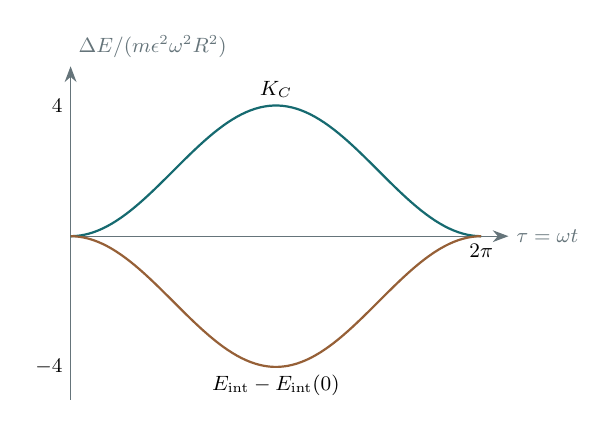
\begin{tikzpicture}[scale=.83,transform shape]

\draw[axis](0,0)--(6.7,0)node[right]{$\tau=\omega t$};\draw[axis](0,-2.5)--(0,2.6)node[above right]{$\Delta E/(m\epsilon^2\omega^2R^2)$};
\draw[traj,domain=0:2*pi,samples=90]plot(\x,{1-cos(deg(\x))});
\draw[thick,color=warm,domain=0:2*pi,samples=90]plot(\x,{-1+cos(deg(\x))});
\node[left]at(0,2){$4$};\node[left]at(0,-2){$-4$};\node[above]at(pi,2){$K_C$};\node[below]at(pi,-2){$E_{\rm int}-E_{\rm int}(0)$};\node[below]at(2*pi,0){$2\pi$};


\end{tikzpicture}
\figcaption{解图电试1.4D\quad 二阶质心动能与内部机械能的相反变化}
\end{minipage}\end{center}



\Needspace{8\baselineskip}

\pdfbookmark[3]{关键洞察}{q4-h5}

\subsection*{关键洞察}

总电荷为零使共同平移产生的磁力相消，内部两速度仍不同，因而其磁力和随时间转动。质心动能所增加的量由内部机械能减少提供；两粒子各自的磁力功始终为零。相对方程中的$q\boldsymbol V_C\times\boldsymbol B$把这项内部反馈明确写出。

\Needspace{8\baselineskip}

\pdfbookmark[3]{易错点}{q4-h6}

\subsection*{易错点}

\begin{itemize}
\item 正、负电荷的速度与电荷符号同时反向，初始两磁力同向。
\item 求质心加速度使用总质量$2m$；分量方程中的系数为$q\omega RB/m$。
\item 正弦外力积分产生$1-\cos\omega t$，常量项决定水平方向的平均速度。
\item 内部零阶圆运动用于求一阶质心位移；二阶能量由同阶内部变化配合。
\item 本题给定静磁场中的初态，建场感应冲量按题设忽略。
\end{itemize}

\Needspace{8\baselineskip}

\pdfbookmark[3]{课堂讲解建议}{q4-h7}

\subsection*{课堂讲解建议}

先让学生在题图标出两速度、两磁力，说明总力为什么向上。积分到$v_{Cx}$后，把常量项与余弦项分别画出，让学生读出初始相消及半周期同向。将图B分成匀速圆心和旋转半径，求周期末的位移与速度。随后用$A=\epsilon R$比较图C的两个长度尺度，再沿图D分别计算整体和内部功率，由两个相反的三重积说明能量如何交换。

\Needspace{8\baselineskip}

\pdfbookmark[3]{变式训练}{q4-h8}

\subsection*{变式训练}

\begin{enumerate}
\Needspace{34\baselineskip}
\item 把磁场方向改为$-z$，初始内部位置、速度均保持。求质心运动，并说明几何方向。
\textbf{解：}图V1中两个初始磁力均向下。用有符号$A=qB_zR/(m\omega)$写主解，$B_z=-B$使$A$变号，故
\[X_C=-A_0(\tau-\sin\tau),\quad Y_C=-A_0(1-\cos\tau),\qquad A_0=\frac{qBR}{m\omega}>0.\]
轨迹关于原点转180度，平均漂移向左、第一拱向下。内部零阶角频率由库仑引力给出，保持原值。两磁力和的方向随$B_z$反向，质心速率与动能则在该阶保持相同大小。
\begin{center}\begin{minipage}{.98\linewidth}\centering
\begin{tikzpicture}[scale=.83,transform shape]
\draw[axis](-4,0)--(4,0)node[right]{$X_C$};\draw[axis](0,-2)--(0,2)node[above]{$Y_C$};\draw[traj,domain=0:2*pi,samples=75]plot({.5*(\x-sin(deg(\x)))},{.7*(1-cos(deg(\x)))});\draw[thick,color=warm,domain=0:2*pi,samples=75]plot({-.5*(\x-sin(deg(\x)))},{-.7*(1-cos(deg(\x)))});\node at(2,1.8){$B_z>0$};\node at(-2,-1.8){$B_z<0$};
\end{tikzpicture}
\figcaption{变图电试1.4V1}
\end{minipage}\end{center}

\Needspace{34\baselineskip}
\item 求第一周期的最高点和再次零速点的位置、时间及速度，比较两种状态。
\textbf{解：}图V2中$Y_C=A(1-\cos\tau)$在$\tau=\pi$达到$2A$，此时
\[t=\pi/\omega,\quad (X_C,Y_C)=(\pi A,2A),\quad
(v_{Cx},v_{Cy})=(2A\omega,0).\]
竖直速度在最高点由正转负，水平方向仍继续前进。到$\tau=2\pi$，两速度同时为零，位置为$(2\pi A,0)$，形成下一个尖点。图V2的水平速度箭头标在最高点，零速度标在尖点，两处由不同分量条件确定。
\begin{center}\begin{minipage}{.98\linewidth}\centering
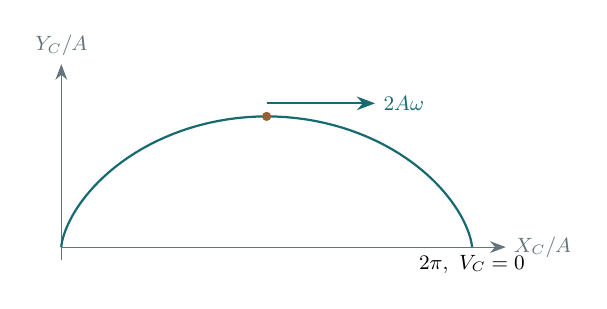
\begin{tikzpicture}[scale=.83,transform shape]
\draw[axis](0,0)--(6.8,0)node[right]{$X_C/A$};\draw[axis](0,-.2)--(0,2.8)node[above]{$Y_C/A$};\draw[traj,domain=0:2*pi,samples=85]plot({\x-sin(deg(\x))},{1-cos(deg(\x))});\fill[warm](pi,2)circle(2pt);\draw[motion](pi,2.2)--(4.8,2.2)node[right]{$2A\omega$};\node[below]at(2*pi,0){$2\pi,\ V_C=0$};
\end{tikzpicture}
\figcaption{变图电试1.4V2}
\end{minipage}\end{center}

\Needspace{34\baselineskip}
\item 系统增加共同水平初速度$V_0\hat x$，仍以相同内部圆运动准备初态。求关于$B$的一阶质心运动，并指出内部磁反馈的阶次。
\textbf{解：}图V3中共同速度在总磁力中仍相消。积分时保留初速度，得
\[X_C=V_0t+A(\tau-\sin\tau),\qquad Y_C=A(1-\cos\tau).\]
一般的内部方程含$(q/m)\boldsymbol V_C\times\boldsymbol B$，初始$V_0$在其中给一阶项，因此内部轨迹已有$O(B)$修正。将这项内部速度修正再乘$B$，对质心的影响从二阶进入，所以有限时间内的一阶质心式仍由零阶圆运动求得。若要求内部轨迹也保持到一阶精度，则相应地计入该强迫项；$V_0=O(B)$时内部反馈回到二阶。
\begin{center}\begin{minipage}{.98\linewidth}\centering
\begin{tikzpicture}[scale=.83,transform shape]
\draw[axis](0,0)--(7.2,0)node[right]{$X_C/A$};\draw[axis](0,0)--(0,2.5)node[above]{$Y_C/A$};\draw[traj,domain=0:2*pi,samples=85]plot({.5*(2*\x-sin(deg(\x)))},{1-cos(deg(\x))});\node[above]at(3.5,2.1){示例 $V_0=A\omega$};\node[below]at(3.5,-.5){增加共同初速后，初始点带有水平速度};
\end{tikzpicture}
\figcaption{变图电试1.4V3}
\end{minipage}\end{center}

\Needspace{34\baselineskip}
\item 在某时刻测得正电荷相对质心的位置为$(r_x,r_y)$。初态仍为$(0,-R)$且质心静止，求该时刻的精确质心速度，再代入零阶圆运动。
\textbf{解：}图V4用内部位移指向当前正电荷。把$m\dot{\boldsymbol V}_C=q\dot{\boldsymbol r}\times\boldsymbol B$积分，
\[m\boldsymbol V_C=q[\boldsymbol r(t)-\boldsymbol r(0)]\times\boldsymbol B,
\quad V_{Cx}=\frac{qB}{m}(r_y+R),\quad V_{Cy}=-\frac{qB}{m}r_x.\]
若取$r_x=-R\sin\tau,r_y=-R\cos\tau$，得到主解速度。此关系在静磁场中直接来自精确总力方程，内部轨道有所改变时仍适用；不同近似只体现在所代入的内部位置。
\begin{center}\begin{minipage}{.98\linewidth}\centering
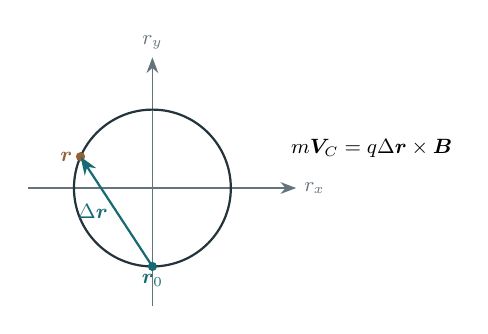
\begin{tikzpicture}[scale=.83,transform shape]
\draw[axis](-1.9,0)--(2.2,0)node[right]{$r_x$};\draw[axis](0,-1.8)--(0,2)node[above]{$r_y$};\draw[object](0,0)circle(1.2);\fill[accent](0,-1.2)circle(2pt)node[below]{$\boldsymbol r_0$};\fill[warm](-1.1,.48)circle(2pt)node[left]{$\boldsymbol r$};\draw[motion](0,-1.2)--(-1.1,.48)node[midway,left]{$\Delta\boldsymbol r$};\node[right]at(2,.6){$m\boldsymbol V_C=q\Delta\boldsymbol r\times\boldsymbol B$};
\end{tikzpicture}
\figcaption{变图电试1.4V4}
\end{minipage}\end{center}

\Needspace{34\baselineskip}
\item 初始内部相位改为$\alpha$，正电荷位置为$-R(\sin\alpha,\cos\alpha)$，仍顺时针转动且质心静止。求一阶质心轨迹及每周期漂移。
\textbf{解：}图V5的内部位置角整体转过$-\alpha$。由上题位移关系，积分得到
\[X_C=A[\tau\cos\alpha-\sin(\tau+\alpha)+\sin\alpha],\]
\[Y_C=A[\cos\alpha-\cos(\tau+\alpha)-\tau\sin\alpha].\]
周期末位移为$2\pi A(\cos\alpha,-\sin\alpha)$，平均速度为$A\omega(\cos\alpha,-\sin\alpha)$。轨迹是主解摆线整体旋转$-\alpha$后的结果，仍从零速度尖点出发。初始相位决定平均漂移的方向，速率的周期变化和最大值保持相同。
\begin{center}\begin{minipage}{.98\linewidth}\centering
\begin{tikzpicture}[scale=.83,transform shape]
\draw[axis](-.2,0)--(5.3,0)node[right]{$X_C/A$};\draw[axis](0,-4.7)--(0,2.3)node[above]{$Y_C/A$};\draw[traj,domain=0:2*pi,samples=90]plot({cos(45)*(\x-sin(deg(\x)))+sin(45)*(1-cos(deg(\x)))},{-sin(45)*(\x-sin(deg(\x)))+cos(45)*(1-cos(deg(\x)))});\node[right]at(.5,1.8){$\alpha=45^\circ$};\draw[motion](2.8,-2.8)--(4.1,-4.1)node[right]{平均漂移};
\end{tikzpicture}
\figcaption{变图电试1.4V5}
\end{minipage}\end{center}

\Needspace{34\baselineskip}
\item 两电荷仍为$\pm q$，质量改为$m_+,m_-$，初始间距为$d$，绕静止质心作库仑圆运动。求一阶质心运动的尺度。
\textbf{解：}图V6中两轨道半径为$m_-d/M$与$m_+d/M$，$M=m_++m_-$，约化质量$\mu=m_+m_-/M$。相对圆运动有
\[\omega^2=\frac{q^2}{4\pi\varepsilon_0\mu d^3},\qquad
M\dot{\boldsymbol V}_C=q\dot{\boldsymbol d}\times\boldsymbol B.\]
取初始$\boldsymbol d=(0,-d)$，零阶圆运动代入后得到与主解同形的摆线，尺度
\[A=\frac{qBd}{M\omega},\quad X_C=A(\tau-\sin\tau),\quad Y_C=A(1-\cos\tau).\]
两质量相等时$d=2R$，回到主解。质量不等时，内部相对方程还有$q(1/m_+-1/m_-)\dot{\boldsymbol d}\times\boldsymbol B$的一阶项；该项对质心结果的反馈从再乘$B$后的二阶进入。
\begin{center}\begin{minipage}{.98\linewidth}\centering
\begin{tikzpicture}[scale=.83,transform shape]
\draw[axis](0,-2)--(0,1.8)node[above]{$y$};\fill[accent](0,-1.5)circle(3pt)node[left]{$m_+,+q$};\fill[warm](0,.75)circle(3pt)node[left]{$m_-,-q$};\fill(0,0)circle(1.5pt)node[right]{$C$};\draw[<->,thin,color=muted](.6,-1.5)--(.6,.75)node[midway,right]{$d$};\draw[motion](0,-1.5)--(-1,-1.5);\draw[motion](0,.75)--(.7,.75);\node[right]at(1.6,0){示例 $m_-:m_+=2:1$};
\end{tikzpicture}
\figcaption{变图电试1.4V6}
\end{minipage}\end{center}

\Needspace{34\baselineskip}
\item 说明一个完整内部周期的总外力冲量和质心净位移，求第一半周期、第二半周期的质心动量变化。
\textbf{解：}图V7中$V_{Cx}=A\omega(1-\cos\tau)\ge0$，因此质心在整个周期持续向右前进。两半周期的动量变化分别为
\[\Delta\boldsymbol P_1=4mA\omega\hat x,\qquad
\Delta\boldsymbol P_2=-4mA\omega\hat x,\]
总冲量为零，周期初末质心速度同为零。位移由速度积分，仍为$2\pi A\hat x$，平均速度为$A\omega\hat x$。两阶段的冲量抵消对应动量恢复，速度曲线下的正面积则对应非零前进距离。
\begin{center}\begin{minipage}{.98\linewidth}\centering
\begin{tikzpicture}[scale=.83,transform shape]
\draw[axis](0,0)--(6.7,0)node[right]{$\tau$};\draw[axis](0,-.2)--(0,2.6)node[above right]{$V_{Cx}/(A\omega)$};\fill[accent!10](0,0)--plot[domain=0:2*pi,samples=70](\x,{1-cos(deg(\x))})--(2*pi,0)--cycle;\draw[traj,domain=0:2*pi,samples=70]plot(\x,{1-cos(deg(\x))});\draw[guide](pi,0)--(pi,2);\node[below]at(pi,0){$\pi$};\node[below]at(2*pi,0){$2\pi$};\node at(pi,1){正面积 $2\pi$};
\end{tikzpicture}
\figcaption{变图电试1.4V7}
\end{minipage}\end{center}

\Needspace{34\baselineskip}
\item 求质心从初始尖点出发时的小时间轨迹，消去时间得到尖点附近的几何关系。
\textbf{解：}图V8放大$\tau\ll1$的第一拱。展开正弦、余弦，
\[X_C=A\left(\frac{\tau^3}{6}-\frac{\tau^5}{120}+\cdots\right),\qquad
Y_C=A\left(\frac{\tau^2}{2}-\frac{\tau^4}{24}+\cdots\right).\]
初始向上加速度为$A\omega^2=qB\omega R/m$，水平位移从$t^3$出现。取最低非零阶消去$\tau$，得$Y_C^3=(9A/2)X_C^2$。所以尖点的切线沿$+y$，随后的水平位移逐渐积累，整个拱仍向右展开。两坐标的不同起始幂次直接来自初始总力向上及其随时间转动。
\begin{center}\begin{minipage}{.98\linewidth}\centering
\begin{tikzpicture}[scale=.83,transform shape]
\draw[axis](0,0)--(2.4,0)node[right]{$X_C/A$};\draw[axis](0,-.1)--(0,3.3)node[above]{$Y_C/A$};\draw[traj,domain=0:1,samples=60]plot({10*(\x-sin(deg(\x)))},{6*(1-cos(deg(\x)))});\node[below]at(1,-.6){示尖点邻域，横纵比例分别放大};\draw[motion](0,.1)--(0,.9);
\end{tikzpicture}
\figcaption{变图电试1.4V8}
\end{minipage}\end{center}
\end{enumerate}

\Needspace{13\baselineskip}

\pdfbookmark[2]{第 5 题 带电容滑动双棒的充电与最终速度}{q5}

\section*{第 5 题\quad 带电容滑动双棒的充电与最终速度}\label{q:5}


两条水平、足够长的平行导轨上有左右两根可无摩擦滑动的导体棒。每根棒长度$l$、质量$m$、电阻$R$，棒中各串接一个电容为$C$的相同电容器，两个电容器初始均未充电；导轨电阻可忽略，组成矩形回路。均匀静磁场$B$垂直回路平面向内。初始左棒静止，右棒以$v_0>0$沿导轨向右运动，初始棒间距$d_0$有限，所有辐射与回路自感忽略。
\begin{enumerate}
\item 对电容$C$的充电过程，能否用静止回路等效：保持两棒的电阻$R$及两电容$C$，再串联一个电容$C'$与恒定电源$\mathcal E'$，于$t=0$闭合？若能，求$\mathcal E',C'$。
\item 求两棒速度、电容电荷随时间的关系。
\item 求两棒最终速度，说明是否相等；带电容时棒间距是否趋向有限值？
\item 将两个电容器取去、用导线接通相应断点，求此时最终速度和棒间距的极限。
\end{enumerate}


\begin{center}\begin{minipage}{.98\linewidth}\centering
\begin{tikzpicture}[scale=.9,transform shape]

\draw[object] (-.6,0)--(5,0);\draw[object] (-.6,2.7)--(5,2.7);
\foreach \x in {0,4}{
\draw[object] (\x,0)--(\x,.95);
\draw[object,line width=1pt] (\x-.36,.95)--(\x+.36,.95);
\draw[object,line width=1pt] (\x-.36,1.15)--(\x+.36,1.15);
\draw[object] (\x,1.15)--(\x,1.8);
\draw[object] (\x-.14,1.8) rectangle (\x+.14,2.35);
\draw[object] (\x,2.35)--(\x,2.7);
\node[right] at (\x+.5,1.05) {$C$};
\node[right] at (\x+.2,2.08) {$R$};
}
\node at (2,1.6) {$\otimes\ B$};
\draw[axis,<->] (-.9,0)--(-.9,2.7) node[midway,left] {$l$};
\draw[motion] (4.15,3.2)--(5.4,3.2) node[midway,above] {$v_0$};
\node[above] at (0,3) {初始静止};
\draw[axis,<->] (0,-.5)--(4,-.5) node[midway,below] {$d_0$};

\end{tikzpicture}
\figcaption{图电试1.5\quad 两棒各串一个C、各有电阻R；初始电容均不带电。}
\end{minipage}\end{center}

\Needspace{8\baselineskip}

\pdfbookmark[3]{题型定位}{q5-h0}

\subsection*{题型定位}

以累计电荷$Q$连接电路与两棒动力学，先把速度写为$Q$的函数，再得到闭合充电方程。图B的附加串联电容表示机械反馈。求完时间历程后，分别讨论有电容、接通断点两种状态的速度与间距，并用能量分配解释充电过程。

\Needspace{8\baselineskip}

\pdfbookmark[3]{知识点}{q5-h1}

\subsection*{知识点}

\begin{itemize}
\item 运动电动势由两棒的速度差给出，电阻总量为$2R$、电容电压总量为$2Q/C$。
\item 安培冲量为$\pm BlQ$，两棒水平总动量守恒，质心速度保持$v_0/2$。
\item 机械速度反馈给充电方程增加$2B^2l^2Q/m$，对应$C'=m/(2B^2l^2)$。
\item 充电时间常量为$CR/(1+\eta)$，最终电容电压与非零运动电动势平衡。
\item 棒间距由相对速度的积分决定，能量按质心、相对运动、电容和焦耳热分配。
\end{itemize}

\Needspace{8\baselineskip}

\pdfbookmark[3]{物理图像}{q5-h2}

\subsection*{物理图像}

题图标出两只电容、两棒电阻与向内磁场。图A的逆时针电流使右棒向左受力、左棒向右受力，两力相消。图B将机械反馈画成第三个串联电容。图C的两速度平台间保留$v_0/(1+\eta)$，对应非零运动电动势。图D在接通断点后画出指数速度差及其面积，速度差趋零时只积累有限分离距离。

\Needspace{8\baselineskip}

\pdfbookmark[3]{解题入口}{q5-h3}

\subsection*{解题入口}

在图A上同时写两棒的安培力和回路电压，按$I\dd t=\dd Q$积分出速度。将两速度代回电动势后，电荷成为唯一未知函数；与图B逐项对应，求附加电容及电源。随后以积分因子求$Q(t)$，再恢复两棒速度和间距。终态从$I\to0$后的电压分配求出。

\Needspace{8\baselineskip}

\pdfbookmark[3]{标准解法}{q5-h4}

\subsection*{标准解法}


图电试1.5规定两棒速度向右为正，记右棒$v_r$、左棒$v_l$；回路电流$I$取逆时针为正。右棒向右时，棒内正电荷所受$\boldsymbol v\times\boldsymbol B$向上，沿逆时针产生正电动势；左棒后来也向右运动，在同一绕行方向中产生相反的电动势。两项相减，使驱动取决于两棒的相对速度。按此方向定义电容电荷$Q(t)=\int_0^t I(t')\,\mathrm dt'$，两个相同电容串联，电压降之和为$2Q/C$。
相对运动产生的总电动势与回路方程为
\[
\mathcal E=Bl(v_r-v_l),\qquad
\boxed{Bl(v_r-v_l)=\frac{2Q}{C}+2RI},\qquad I=\dot Q.
\]
图A中右棒电流向上，安培力向左；左棒电流向下，安培力向右。两力大小相等，水平总动量保持不变。以逆时针电流$I$为同一个累计量，两棒动力学为
\[
m\dot v_r=-BlI,\qquad m\dot v_l=+BlI.
\]
\begin{center}\begin{minipage}{.98\linewidth}\centering
\begin{tikzpicture}[scale=.75,transform shape]

\draw[object] (-.6,0)--(5,0);\draw[object] (-.6,2.7)--(5,2.7);
\foreach \x in {0,4}{
\draw[object] (\x,0)--(\x,.95);
\draw[object,line width=1pt] (\x-.36,.95)--(\x+.36,.95);
\draw[object,line width=1pt] (\x-.36,1.15)--(\x+.36,1.15);
\draw[object] (\x,1.15)--(\x,1.8);
\draw[object] (\x-.14,1.8) rectangle (\x+.14,2.35);
\draw[object] (\x,2.35)--(\x,2.7);
\node[right] at (\x+.5,1.05) {$C$};
\node[right] at (\x+.2,2.08) {$R$};
}
\node at (2,1.6) {$\otimes\ B$};
\draw[axis,<->] (-.9,0)--(-.9,2.7) node[midway,left] {$l$};
\draw[motion] (4.15,3.2)--(5.4,3.2) node[midway,above] {$v_r$};
\draw[motion] (.15,3.2)--(1.2,3.2) node[midway,above] {$v_l$};
\draw[axis,<->] (0,-.5)--(4,-.5) node[midway,below] {$d$};

\draw[force] (3.8,.45)--(2.7,.45) node[midway,above] {$-BlI$};
\draw[force] (.2,.45)--(1.3,.45) node[midway,above] {$+BlI$};
\draw[motion] (3,2.7)--(1.5,2.7) node[midway,above] {$I$};
\draw[motion] (1.5,0)--(3,0);
\node at (2,-1.3) {$Bl(v_r-v_l)=2Q/C+2RI$};

\end{tikzpicture}
\figcaption{解图电试1.5A\quad 逆时针电流使右棒受阻、左棒加速，总水平力相消。}
\end{minipage}\end{center}
解图电试1.5A把这两个安培力与电流标在同一回路。将$I\,\dd t$写为$\dd Q$，从$Q=0$积分到当前电量：右棒的动量改变量为$-BlQ$，左棒为$+BlQ$。两棒初始动量分别为$mv_0$与0，故
\[
\boxed{v_r=v_0-\frac{Bl}{m}Q,\qquad
v_l=\frac{Bl}{m}Q}.
\]
两速度之和始终为$v_0$，质心速度因此保持$v_0/2$。
将其代入回路方程，得到
\[
\boxed{2R\dot Q+
2\left(\frac1C+\frac{B^2l^2}{m}\right)Q=Blv_0}.
\]
这个附加项来自两棒速度差的减小：每累计电量$\dd Q$，右棒速度减小$(Bl/m)\dd Q$，左棒速度增加同样大小，两者使电动势总共减少$(2B^2l^2/m)\dd Q$。电容充电增大$2Q/C$，机械运动使驱动减小；将它与电容电压放在方程同一侧，得到总的电荷系数。

第（1）问的静止回路含三个串联电容，等效串联电容$C_\Sigma$满足
\[
\frac1{C_\Sigma}=\frac2C+\frac1{C'}.
\]
\begin{center}\begin{minipage}{.98\linewidth}\centering
\begin{tikzpicture}[scale=.85,transform shape]

\draw[object] (0,0)--(0,.9);
\draw[object,line width=1pt] (-.35,.9)--(.35,.9);
\draw[object,line width=1pt] (-.35,1.1)--(.35,1.1);
\draw[object] (0,1.1)--(0,1.7);
\draw[object] (-.14,1.7) rectangle (.14,2.25);
\draw[object] (0,2.25)--(0,2.6)--(1.8,2.6);
\draw[object,line width=1pt] (1.8,2.25)--(1.8,2.95);
\draw[object,line width=1pt] (2,2.25)--(2,2.95);
\draw[object] (2,2.6)--(4,2.6)--(4,2.25);
\draw[object] (3.86,1.7) rectangle (4.14,2.25);
\draw[object] (4,1.7)--(4,1.1);
\draw[object,line width=1pt] (3.65,1.1)--(4.35,1.1);
\draw[object,line width=1pt] (3.65,.9)--(4.35,.9);
\draw[object] (4,.9)--(4,0)--(2.1,0);
\draw[object] (2.1,-.35)--(2.1,.35);
\draw[object] (1.9,-.18)--(1.9,.18);
\draw[object] (1.9,0)--(0,0);
\node[above] at (1.9,3) {$C'$};
\node[left] at (-.4,1) {$C$};\node[right] at (4.4,1) {$C$};
\node[left] at (-.2,2) {$R$};\node[right] at (4.2,2) {$R$};
\node[below] at (2,-.5) {$\mathcal E'=Blv_0$};
\node at (2,-1.2) {三个电容串联；初始均未充电};

\end{tikzpicture}
\figcaption{解图电试1.5B\quad 静止等效回路用附加串联电容表示机械反馈。}
\end{minipage}\end{center}
解图电试1.5B中所有电容初始不带电，回路电流经过两个电阻，总电阻仍为$2R$，充电方程为
\[
2R\dot Q+\left(\frac2C+\frac1{C'}\right)Q=\mathcal E'.
\]
逐项比较同一个$Q(t)$所满足的方程，得到
\[
\boxed{\mathcal E'=Blv_0,\qquad
C'=\frac{m}{2B^2l^2}}.
\]
两个回路有相同的总电阻、相同的初始电量和相同的充电微分方程，因此每个时刻的$Q(t)$与$I(t)$相同。新增串联电容的电压$Q/C'=2B^2l^2Q/m$恰好对应机械反馈项。静止回路的能量由恒定电源供给，运动回路的能量由两棒动能供给，分别按各自供能过程计算。

第（2）问记无量纲耦合与时间尺度
\[
\eta=\frac{CB^2l^2}{m},\qquad
\tau=\frac{CR}{1+\eta},\qquad
Q_\infty=\frac{CBlv_0}{2(1+\eta)}.
\]
由$2RC_\Sigma=\tau$，充电方程化为$\dot Q+Q/\tau=Q_\infty/\tau$。乘积分因子$e^{t/\tau}$，
\[
\frac{\dd}{\dd t}(Qe^{t/\tau})=\frac{Q_\infty}{\tau}e^{t/\tau},\qquad
Q(t)e^{t/\tau}-Q(0)=Q_\infty(e^{t/\tau}-1).
\]
取$Q(0)=0$并求导，得到
\[
\boxed{Q(t)=Q_\infty(1-e^{-t/\tau}),\qquad
I(t)=\frac{Blv_0}{2R}e^{-t/\tau}}.
\]
在两棒速度与电量的关系中代入这条充电曲线。右棒减去累计安培冲量对应的速度，左棒增加同样大小；系数$(Bl/m)Q_\infty$化为$v_0\eta/[2(1+\eta)]$。于是
\[
\boxed{v_r(t)=v_0\left[1-\frac{\eta}{2(1+\eta)}(1-e^{-t/\tau})\right]},
\]
\[
\boxed{v_l(t)=v_0\frac{\eta}{2(1+\eta)}(1-e^{-t/\tau})}.
\]
\begin{center}\begin{minipage}{.98\linewidth}\centering
\begin{tikzpicture}[scale=.85,transform shape]

\draw[axis] (0,0)--(5.5,0) node[right] {$t/\tau$};
\draw[axis] (0,0)--(0,3.9) node[above] {$v/v_0$};
\draw[traj,domain=0:4.5,samples=70] plot (\x,{3.5*(.75+.25*exp(-\x))});
\draw[thick,color=warm,domain=0:4.5,samples=70] plot (\x,{3.5*.25*(1-exp(-\x))});
\draw[guide] (0,2.625)--(4.9,2.625);
\draw[guide] (0,.875)--(4.9,.875);
\node[left] at (0,3.5) {$1$};
\node[left] at (0,2.625) {$3/4$};\node[left] at (0,.875) {$1/4$};
\node[above,color=accent] at (2.5,2.9) {$v_r$};
\node[below,color=warm] at (2.5,.6) {$v_l$};
\node at (2.9,3.9) {示例 $\eta=CB^2l^2/m=1$};

\end{tikzpicture}
\figcaption{解图电试1.5C\quad 带电容时充电结束，两棒速度平台仍有间隔。}
\end{minipage}\end{center}
解图电试1.5C中右棒减速、左棒加速，两者最终有不同平台值：
\[
\boxed{v_{r,\infty}=\frac{2+\eta}{2(1+\eta)}v_0,\qquad
v_{l,\infty}=\frac{\eta}{2(1+\eta)}v_0}.
\]
两棒最终相对速度
\[
w_\infty=v_{r,\infty}-v_{l,\infty}=\frac{v_0}{1+\eta}>0.
\]
充电后期，电阻电压$2RI$趋零，剩余的非零运动电动势由两个电容电压共同抵消，即
\[
Blw_\infty=\frac{2Q_\infty}{C}.
\]
电容电压已经抵消非零的运动电动势，故电流停止、两棒却仍以不同速度运动。相对速度全过程为
\[
w(t)=\frac{v_0}{1+\eta}(1+\eta e^{-t/\tau}),
\]
所以棒间距为
\[
\boxed{d(t)=d_0+\frac{v_0}{1+\eta}
\left[t+\eta\tau(1-e^{-t/\tau})\right]}.
\]
对有限$C>0$，相对速度有正的平台$v_0/(1+\eta)$，其时间积分持续增长，间距渐近线性增大。瞬态指数项只提供有限的附加距离$v_0\eta\tau/(1+\eta)$。因此两棒速度各自趋于有限值，同时棒间距趋于无穷大，这两种极限分别由速度本身和速度的时间积分决定。

第（4）问去掉电容、将断点接通后，方程改为
\[
I=\frac{Blw}{2R},\qquad
\dot w=-\frac{2Bl}{m}I=-\frac{B^2l^2}{mR}w.
\]
记$\tau_0=mR/(B^2l^2)$，则
\[
w=v_0e^{-t/\tau_0},\quad
v_r=\frac{v_0}{2}(1+e^{-t/\tau_0}),\quad
v_l=\frac{v_0}{2}(1-e^{-t/\tau_0}).
\]
\begin{center}\begin{minipage}{.98\linewidth}\centering
\begin{tikzpicture}[scale=.7,transform shape]

\draw[axis] (0,0)--(3.7,0) node[right] {$t/\tau_0$};
\draw[axis] (0,0)--(0,2.9) node[above] {$w/v_0$};
\draw[traj,domain=0:3.3,samples=60] plot (\x,{2.5*exp(-\x)});
\node[left] at (0,2.5) {$1$};
\begin{scope}[xshift=6cm]
\draw[axis] (0,0)--(3.7,0) node[right] {$t/\tau_0$};
\draw[axis] (0,0)--(0,2.9) node[above] {$(d-d_0)/(v_0\tau_0)$};
\draw[traj,domain=0:3.3,samples=60] plot (\x,{2.5*(1-exp(-\x))});
\draw[guide] (0,2.5)--(3.4,2.5);\node[left] at (0,2.5) {$1$};
\end{scope}
\node at (4.4,-1) {无电容：相对速度趋零，间距增长有有限积分};

\end{tikzpicture}
\figcaption{解图电试1.5D\quad 接通断点后的相对运动与间距增量，两者使用同一时间尺度。}
\end{minipage}\end{center}
解图电试1.5D对比接通导线后的结果，两棒相对速度趋零，均趋于$v_0/2$，棒间距只增加有限值
\[
\boxed{d_\infty=d_0+\int_0^\infty w\,\mathrm dt
=d_0+\frac{mRv_0}{B^2l^2}}.
\]

上述有限距离还可直接从左棒的动量变化读出。无电容时，$I=Bl(v_r-v_l)/(2R)$，与$m\dd v_l=BlI\dd t$联立，得到
\[
(v_r-v_l)\dd t=\frac{2mR}{B^2l^2}\dd v_l.
\]
左棒速度从0增至$v_0/2$，两边从初态积分到终态，便给间距增量$[2mR/(B^2l^2)](v_0/2)=mRv_0/(B^2l^2)$。该积分把左棒从0到$v_0/2$的速度变化直接换成两棒的分离距离。图D中相对速度曲线下的有限面积，正是同一个距离增量。

\textbf{能量在两棒、电容与电阻之间的分配。}两个串联电容的电量大小均为$Q$，每个储能$Q^2/(2C)$，总储能为$Q^2/C$。两棒机械功率为$-BlI(v_r-v_l)$，电容储能的变化率为$(2Q/C)I$；将回路方程乘$I$，得到电阻发热率$2RI^2$。合并这三项，即有
\[
\frac{\mathrm d}{\mathrm dt}
\left[\frac m2(v_r^2+v_l^2)+\frac{Q^2}{C}\right]
=-2RI^2.
\]
代入$I(t)$积分，最终焦耳热为
\[
H=2R\int_0^\infty I^2\,\mathrm dt
=\frac{mv_0^2}{4}\frac{\eta}{1+\eta}.
\]
它与最终两棒动能、电容储能相加，恢复初始动能$mv_0^2/2$。恒定磁场的磁力不直接做功，机械能通过运动电动势转为电容能和焦耳热。

还可按质心与相对运动分开这些能量。两棒的质心速度一直为$v_0/2$，故质心动能为$mv_0^2/4$。相对速度为$w$时，相对动能为$mw^2/4$，初始相对动能也为$mv_0^2/4$。最终相对速度为$v_0/(1+\eta)$，因此
\[
K_{\rm rel,\infty}=\frac{mv_0^2}{4(1+\eta)^2},\qquad
U_{C,\infty}=\frac{Q_\infty^2}{C}
=\frac{mv_0^2\eta}{4(1+\eta)^2}.
\]
两项之和为$mv_0^2/[4(1+\eta)]$，与焦耳热$mv_0^2\eta/[4(1+\eta)]$相加，正好等于初始相对动能。质心平动保持，释放出来的相对动能分给电容和电阻。充电量随时间增加，安培力按同一指数衰减；这个过程在电路中表现为电容电压逐渐承担更多的运动电动势，在力学中表现为两棒速度逐渐进入图C的不同平台。

去掉电容后，电路中的运动电动势全部降落在电阻上，相对速度最终趋零，初始相对动能$mv_0^2/4$全部成为焦耳热，质心动能仍保持$mv_0^2/4$。两种电路的长期结果由是否保留稳态电容电压决定：有电容时非零电压配合非零速度差，无电容时电阻电压随电流共同趋零，速度差也趋零。



\Needspace{8\baselineskip}

\pdfbookmark[3]{关键洞察}{q5-h5}

\subsection*{关键洞察}

有电容时，充电完成后的$2Q_\infty/C$维持非零速度差，电流与安培力均趋零。接通断点后，运动电动势只由电阻消耗，速度差随电流一起衰减到零。两种情况的初始电流相同，随后电压在电容和电阻间的分配不同，长期速度与分离距离也随之不同。

\Needspace{8\baselineskip}

\pdfbookmark[3]{易错点}{q5-h6}

\subsection*{易错点}

\begin{itemize}
\item 两棒电动势按同一绕行方向相减，驱动为$Bl(v_r-v_l)$。
\item 两电容串联的电压是$2Q/C$，两棒电阻串联为$2R$。
\item 两安培力等大反向，两速度之和保持$v_0$。
\item 静止等效回路与运动回路具有相同$Q(t)$，能量分别由电源和机械运动供给。
\item 有电容时$I_\infty=0$对应$Blw_\infty=2Q_\infty/C$，保留正的$w_\infty$。
\item 间距由速度差积分求得，有限速度平台给出线性增长的间距。
\end{itemize}

\Needspace{8\baselineskip}

\pdfbookmark[3]{课堂讲解建议}{q5-h7}

\subsection*{课堂讲解建议}

先在图A画电流和两安培力，求出每经过电量$\dd Q$两棒的动量变化，再得到速度与电量关系。讲图B时让学生分别写出每个串联电容的电压，找到机械项与$Q/C'$的对应。用图C的两平台计算最终电容电压和运动电动势。最后接通电容断点，重写回路方程，沿图D计算相对速度曲线下的面积，并把两种情形的质心动能、相对动能、电容储能及焦耳热列在同一组初始能量下。

\Needspace{8\baselineskip}

\pdfbookmark[3]{变式训练}{q5-h8}

\subsection*{变式训练}

\begin{enumerate}
\Needspace{35\baselineskip}
\item 取$\eta=0.10$，求最终两棒速度、时间常量，并写出弱耦合的首阶近似。
\textbf{解：}图V1的左棒只获得较小速度。代入精确式，
\[v_{l,\infty}=\frac{v_0}{22}=0.0454545v_0,\quad
v_{r,\infty}=\frac{21v_0}{22}=0.9545455v_0,\quad \tau=CR/1.10.\]
当$\eta\ll1$时，$1/(1+\eta)=1-\eta+O(\eta^2)$，故$v_{l,\infty}\simeq\eta v_0/2$、$v_{r,\infty}\simeq v_0(1-\eta/2)$、$\tau\simeq CR$。电容在右棒速度变化较小时已接近充满，机械反馈在电荷系数中只占$\eta$的相对份额。
\begin{center}\begin{minipage}{.98\linewidth}\centering
\begin{tikzpicture}[scale=.82,transform shape]
\draw[axis](0,0)--(5,0)node[right]{$t/\tau$};\draw[axis](0,-.1)--(0,3.1)node[above right]{$v/v_0$};\draw[traj,domain=0:4.5,samples=65]plot(\x,{2.7*(1-(1-exp(-\x))/22)});\draw[thick,color=warm,domain=0:4.5,samples=65]plot(\x,{2.7*(1-exp(-\x))/22});\node[left]at(0,2.7){$1$};\node[right]at(4.5,2.7){$v_r$};\node[right]at(4.5,.15){$v_l$};
\end{tikzpicture}
\figcaption{变图电试1.5V1}
\end{minipage}\end{center}

\Needspace{35\baselineskip}
\item 讨论$C\to\infty$的固定时间极限，再比较任意有限大$C$的长期棒间距。
\textbf{解：}固定$B,l,m,R$时，$\eta\to\infty$且$\tau\to\tau_0=mR/(B^2l^2)$。相对速度
\[w_C(t)=\frac{v_0}{1+\eta}(1+\eta e^{-t/\tau})\]
在每个固定$t$趋于$v_0e^{-t/\tau_0}$，对应接通断点的结果。图V2同时画有限大$\eta$仍保留的平台$v_0/(1+\eta)$。因此有限$C$先取$t\to\infty$时，$d_C(t)\to\infty$；先取$C\to\infty$再取长期极限时，间距为$d_0+v_0\tau_0$。两种取值次序对应保留电容电压与接通断点两种长期过程。
\begin{center}\begin{minipage}{.98\linewidth}\centering
\begin{tikzpicture}[scale=.82,transform shape]
\draw[axis](0,0)--(5,0)node[right]{$t/\tau_0$};\draw[axis](0,0)--(0,3)node[above right]{$w/v_0$};\draw[traj,domain=0:4.5,samples=70]plot(\x,{2.5*(1+9*exp(-\x/0.9))/10});\draw[thick,dashed,color=warm,domain=0:4.5,samples=70]plot(\x,{2.5*exp(-\x)});\draw[guide](0,.25)--(4.8,.25);\node[right]at(4.8,.25){$\eta=9$ 平台};\node[above]at(2,2){虚线 $C\to\infty$};
\end{tikzpicture}
\figcaption{变图电试1.5V2}
\end{minipage}\end{center}

\Needspace{35\baselineskip}
\item 去掉电容后，求初始相对动能和最终焦耳热，并比较质心能量。
\textbf{解：}图V3中初始右棒速度$v_0$、左棒为零，质心速度$v_0/2$。初始总动能$mv_0^2/2$由相等的两项组成：
\[K_{C}=mv_0^2/4,\qquad K_{\rm rel,0}=mv_0^2/4.\]
接通断点后$w=v_0e^{-t/\tau_0}$，相对动能按$e^{-2t/\tau_0}$衰减。以$I=Blw/(2R)$计算，
\[H=2R\int_0^\infty I^2\dd t=\frac{mv_0^2}{4}.\]
质心动能保持，初始相对动能全部转为热。带电容表达式$H=(mv_0^2/4)\eta/(1+\eta)$在$\eta\to\infty$也趋于同一能量。
\begin{center}\begin{minipage}{.98\linewidth}\centering
\begin{tikzpicture}[scale=.82,transform shape]
\draw[axis](0,0)--(5,0)node[right]{$t/\tau_0$};\draw[axis](0,-.1)--(0,3.1)node[above right]{$K/(mv_0^2/4)$};\draw[traj](0,2)--(4.5,2)node[right]{$K_C$};\draw[thick,color=warm,domain=0:4.5,samples=65]plot(\x,{2*exp(-2*\x)});\node[right]at(3,.35){$K_{\rm rel}$};\node[left]at(0,2){$1$};
\end{tikzpicture}
\figcaption{变图电试1.5V3}
\end{minipage}\end{center}

\Needspace{35\baselineskip}
\item 将两电容改为$C_1,C_2$，两棒质量和电阻仍相同，求充电方程、时间常量和等效附加电容。
\textbf{解：}图V4中串联电量仍同为$Q$，总电容电压为$Q/C_1+Q/C_2$。两棒的安培冲量与主解相同，故
\[2R\dot Q+KQ=Blv_0,\qquad
K=\frac1{C_1}+\frac1{C_2}+\frac{2B^2l^2}{m}.\]
由$Q(0)=0$，$Q(t)=(Blv_0/K)(1-e^{-Kt/(2R)})$，时间常量为$2R/K$。静止等效回路的第三电容只表示机械反馈，因此$C'=m/(2B^2l^2)$保持。电能则为$Q^2/(2C_1)+Q^2/(2C_2)$，按两电容各自的电压计算。
\begin{center}\begin{minipage}{.98\linewidth}\centering
\begin{tikzpicture}[scale=.82,transform shape]
\draw[object](0,0)--(0,.8);\draw[object](-.35,.8)--(.35,.8);\draw[object](-.35,1)--(.35,1);\draw[object](0,1)--(0,2)--(4,2)--(4,1);\draw[object](3.65,1)--(4.35,1);\draw[object](3.65,.8)--(4.35,.8);\draw[object](4,.8)--(4,0)--(0,0);\node[left]at(-.4,.9){$C_1$};\node[right]at(4.4,.9){$C_2$};\node[above]at(2,2.2){两棒仍各有 $m,R$};\node at(2,1){$\otimes B$};
\end{tikzpicture}
\figcaption{变图电试1.5V4}
\end{minipage}\end{center}

\Needspace{35\baselineskip}
\item 两棒质量改为$m_r,m_l$，电阻仍各为$R$，电容仍各为$C$，其余初态相同。求等效第三电容和最终速度差。
\textbf{解：}图V5中两棒接受相反的相同冲量，速度为$v_r=v_0-BlQ/m_r$、$v_l=BlQ/m_l$。设$\mu=m_rm_l/(m_r+m_l)$，则
\[2R\dot Q+KQ=Blv_0,\quad K=\frac2C+\frac{B^2l^2}{\mu},\quad
C'=\frac{\mu}{B^2l^2}.\]
所以$Q_\infty=Blv_0/K$、$w_\infty=v_0(2/C)/K>0$，两极限速度分别由上述冲量关系代入$Q_\infty$得到。总动量$m_rv_r+m_lv_l=m_rv_0$保持。取$m_r=m_l=m$时，$\mu=m/2$，恢复主解。
\begin{center}\begin{minipage}{.98\linewidth}\centering
\begin{tikzpicture}[scale=.82,transform shape]
\draw[object](0,0)--(0,2.3);\draw[object](4,0)--(4,2.3);\draw[object](-.5,0)--(5,0);\draw[object](-.5,2.3)--(5,2.3);\node[above]at(0,2.5){$m_l$};\node[above]at(4,2.5){$m_r$};\draw[force](.2,.7)--(1.4,.7)node[midway,above]{$+BlI$};\draw[force](3.8,.7)--(2.6,.7)node[midway,above]{$-BlI$};\node at(2,1.5){$\otimes B$};\node[below]at(2,-.6){相同冲量，不同质量给出不同速度变化};
\end{tikzpicture}
\figcaption{变图电试1.5V5}
\end{minipage}\end{center}

\Needspace{35\baselineskip}
\item 在$B,l,m,R,v_0$固定时改变两个相同电容的电容$C$，求最终总储能的最大值。
\textbf{解：}图V6按$\eta=CB^2l^2/m$横向比较。由
\[U_C=\frac{mv_0^2}{4}\frac{\eta}{(1+\eta)^2},\qquad
\frac{\dd}{\dd\eta}\frac{\eta}{(1+\eta)^2}
=\frac{1-\eta}{(1+\eta)^3},\]
最大值在$\eta=1$，即$C=m/(B^2l^2)$，且$U_{C,\max}=mv_0^2/16$。此时$Q_\infty=mv_0/(4Bl)$，两棒最终速度为$3v_0/4,v_0/4$。图V6曲线在小电容时储能随$C$增加，大电容时机械速度差已显著减小，最终储能反而下降。
\begin{center}\begin{minipage}{.98\linewidth}\centering
\begin{tikzpicture}[scale=.82,transform shape]
\draw[axis](0,0)--(5.5,0)node[right]{$\eta$};\draw[axis](0,-.1)--(0,2.8)node[above right]{$U_C/(mv_0^2/4)$};\draw[traj,domain=0:5,samples=85]plot(\x,{8*\x/(1+\x)^2});\draw[guide](1,0)--(1,2);\fill[warm](1,2)circle(2pt);\node[below]at(1,0){$1$};\node[left]at(0,2){$1/4$};
\end{tikzpicture}
\figcaption{变图电试1.5V6}
\end{minipage}\end{center}

\Needspace{35\baselineskip}
\item 仅将磁场改为垂直平面向外，电流仍以逆时针为正，求充电极性和两棒速度的变化。
\textbf{解：}图V7中有向磁场系数从$B$变为$-B$，充电驱动$Blv_0$反号，而电荷系数只含$B^2$。所以$Q(t),I(t)$均反号，两电容极性反转。安培冲量含乘积$BlQ$，保持原值，两棒的$v_r(t),v_l(t)$与间距均保持。附加电容$C'=m/(2B^2l^2)$和时间常量不变，等效电源$\mathcal E'$反号；储能与焦耳热仍由平方量给出相同数值。
\begin{center}\begin{minipage}{.98\linewidth}\centering
\begin{tikzpicture}[scale=.82,transform shape]
\draw[object](0,0)rectangle(4,2.3);\node at(2,1.4){$\odot B$};\draw[motion](4.2,2.8)--(5.5,2.8)node[midway,above]{$v_0$};\draw[motion](1.2,2.3)--(2.8,2.3)node[midway,above]{电流顺时针};\draw[force](.2,.6)--(1.3,.6);\draw[force](3.8,.6)--(2.7,.6);\node[below]at(2,-.6){电流反向，安培力仍使右棒减速、左棒加速};
\end{tikzpicture}
\figcaption{变图电试1.5V7}
\end{minipage}\end{center}

\Needspace{35\baselineskip}
\item 在静止等效回路中求电源总功和新增电容$C'$的最终储能，说明它们与运动回路机械能变化的联系。
\textbf{解：}图V8中恒定电源通过总电量$Q_\infty$，所做功为$W'=Blv_0Q_\infty$，新增电容储能为
\[U_{C'}=\frac{Q_\infty^2}{2C'}=\frac{B^2l^2Q_\infty^2}{m}.\]
运动回路的两棒动能由$v_r=v_0-BlQ/m,v_l=BlQ/m$展开，其减少量为$Blv_0Q-B^2l^2Q^2/m$。因此最终机械能减少$\Delta K=W'-U_{C'}$，供给原两电容储能和焦耳热。两个回路具有相同$I(t)$，故电阻发热相同；静止回路将额外的$U_{C'}$储存在第三电容。图V8以$\eta=1$为例，按$mv_0^2$归一，$W'=1/4$、$U_{C'}=1/16$、$\Delta K=3/16$、原两电容储能$1/16$、焦耳热$1/8$。
\begin{center}\begin{minipage}{.98\linewidth}\centering
\begin{tikzpicture}[scale=.82,transform shape]
\draw[axis](0,0)--(7,0);\draw[axis](0,0)--(0,3.2)node[above right]{能量$/mv_0^2$};\foreach \x/\h/\lab in{1/2.5/{$W^\prime$},2.3/.625/{$U_{C^\prime}$},3.6/1.875/{$\Delta K$},4.9/.625/{$U_C$},6.2/1.25/{$H$}}{\fill[accent!15](\x-.3,0)rectangle(\x+.3,\h);\draw[object](\x-.3,0)rectangle(\x+.3,\h);\node[below]at(\x,-.1){\lab};}\node[left]at(0,2.5){$1/4$};\node at(3.5,3){示例 $\eta=1$};
\end{tikzpicture}
\figcaption{变图电试1.5V8}
\end{minipage}\end{center}
\end{enumerate}

\end{document}
